\documentclass[10pt,a4paper]{book}
\usepackage[utf8]{inputenc}
\usepackage[portuguese]{babel}
\usepackage[T1]{fontenc}
\usepackage{amsmath,amsthm}
\usepackage{amsfonts}
\usepackage{amssymb}
\usepackage[shortlabels]{enumitem}
\usepackage{multicol}
\usepackage{float} 
\usepackage[all]{xy}
\usepackage[usenames,dvipsnames]{color}
\usepackage{xcolor}
\usepackage{colortbl}
\usepackage{gensymb} % \degree

\definecolor{rosa}{HTML}{edaae5} %para fórmulas
\definecolor{azul}{HTML}{aae5ed} %para definições
\definecolor{amarelo}{HTML}{e5edaa} %para observações importantes
\definecolor{cinza}{HTML}{c6c9c5} %para linhas das tabelas
\definecolor{verde}{HTML}{c4edaa}

\usepackage{graphicx}
%\usepackage[left=2cm,right=2cm,top=2cm,bottom=2cm]{geometry}

%\graphicspath{./Capitulos/Figuras/}

\theoremstyle{definition}
\newtheorem{exem}{Exemplo}
\newcommand{\exemautorefname}{Exemplo}
\newtheorem{obs}{Observação}
\newcommand{\obsautorefname}{Observação}

\theoremstyle{plain}
\newtheorem{defi}{Definição}[section]

\newcommand{\fim}{\hfill {$\Box$}}
\newcommand{\N}{\mathbb{N}}
\newcommand{\Z}{\mathbb{Z}}
\newcommand{\Q}{\mathbb{Q}}
\newcommand{\I}{\mathbb{I}}
\newcommand{\R}{\mathbb{R}}
\newcommand{\C}{\mathbb{C}}
\newcommand{\iu}{{i\mkern1mu}} %unidade imaginária
\newcommand{\sen}{\operatorname{sen}}
\newcommand{\cotan}{\operatorname{cot}}
\newcommand{\cosec}{\operatorname{csc}}
\newcommand{\arcsen}{\operatorname{arcsen}}
\newcommand*\abs[1]{\left|#1\right|}



\newcommand{\azul}{\ensuremath{\blacksquare}}
\newcommand{\destaque}[1]{\colorbox{rosa}{$\displaystyle #1$}}

\author{Francieli Triches}
\title{Materiais}

\begin{document}
\chapter{Análise Combinatória}

Análise combinatória é a área da matemática dedicada aos processos de contagem. É nela que encontramos as ferramentas para contar o número de possibilidades de agrupar e organizar elementos de grupos finitos sobre determinadas circunstâncias.

Um exemplo de um problema de contagem é:
\begin{exem}\label{escnum}
 Quantos números diferentes, sem algarismos repetidos, podemos escrever usando os algarismos $\{4,5,6\}$?

 \underline{Resolução:}

 Para facilitar a compreensão da análise do número de possibilidades vamos usar os seguintes esquemas, chamados árvores de possibilidade:
 \begin{displaymath}
    \xymatrix{4 \ar[dd] \ar[r] \ar[dr] &  5 \\
                & 6 \ar[d] \\
                \text{1 possibilidade} & \text{2 possibilidades} \\
              5 \ar[dd] \ar[r] \ar[dr] & 4 \\
                & 6 \ar[d] \\
                \text{1 possibilidade} & \text{2 possibilidades}}
 \end{displaymath}

 \begin{displaymath}
    \xymatrix{ 6 \ar[dd] \ar[r] \ar[dr] &  4 \\
                & 5 \ar[d] \\
                \text{1 possibilidade} \ar[d] & \text{2 possibilidades} \ar[d] \\
                \text{3 possibilidades} & \text{2 possibilidades}}
\end{displaymath}
Portanto o total de possibilidades é $3 \cdot 2=6$ que como podemos observar é exatamente o número de linhas que temos na 2ª coluna.

Observe que as possibilidades são as seguintes $\{45, 46, 54, 56, 64, 65\}$.

\fim
\end{exem}

Este e outros problemas de contagem, por vezes com condições mais complexas, podem ser resolvidos por meio da análise combinatória, cujas principais ferramentas são princípio fundamental da contagem, fatorial, permutações, arranjos e combinações. Sendo que permutações, arranjos e combinações podem ser simples ou com elementos repetidos.

\section{Princípio fundamental da contagem}

 \vskip0.3cm
 \colorbox{azul}{
 \begin{minipage}{0.9\linewidth}
 \begin{center}
  Se um evento é composto por duas etapas sucessivas e independentes de tal maneira que o número de possibilidades na primeira etapa é $m$ e para cada possibilidade da primeira etapa o número de possibilidades na segunda etapa é $n$, então o número total de possibilidades de o evento ocorrer é dado pelo produto $m \cdot n$.
 \end{center}
 \end{minipage}}
 \vskip0.3cm

No exemplo \ref{escnum} acima queremos contar quantos números diferentes podemos escrever usando os algarismos $\{4,5,6\}$. Este é um exemplo que pode ser resolvido usando o princípio fundamental da contagem. Neste caso, a primeira etapa é o 1º algarismo utilizado para formar o número, para o qual temos $3$ possibilidades de escolha. A segunda etapa é o 2º algarismo utilizado para formar o número, que como não pode repetir algarismos, por exemplo não é permitido formar o número $44$, após cada escolha do 1º algarismo sobram então $2$ algarismos, como possibilidades de escolha para a 2º etapa, que é o 2º algarismo. Logo o número total de possibilidades de o evento ocorrer é dado pelo produto $3 \cdot 2= 6$, como vimos no exemplos \ref{escnum}.

\begin{obs}
 O produto do número de possibilidades vale para qualquer número de etapas independentes.
\end{obs}


\section{Fatorial}

\vskip0.3cm
 \colorbox{azul}{
 \begin{minipage}{0.9\linewidth}
 \begin{center}
  O fatorial de um número natural $n$, representado por $n!$, é o produto de todos os inteiros positivos menores ou iguais a $n$, ou seja,
 \[n! = n.(n-1).(n-2)...3.2.1. \]
 \end{center}
 \end{minipage}}
 \vskip0.3cm

 Considera-se $\destaque{0!= 1}$ e $\destaque{1!= 1}$.


\section{Permutações}

Dado um conjunto com $n$ elementos, o ato de organizar estes elementos ordenando-os, de forma que cada nova ordem é considerada como um novo elemento é chamado de permutação. Existem dois tipos de permutação, a permutação simples quando os $n$ elementos são distintos, e a permutação com repetição quando no conjuntos de $n$ elementos temos elementos repetidos.

\subsection{Permutação simples}

Dados $n$ elementos distintos, vejamos como calcular quantos agrupamentos é possível formar usando os $n$ elementos.
\begin{exem}
 Quantos números de 3 algarismo (sem repeti-los num mesmo número) podemos formar com os algarismos $2, 4, 8$?

 \underline{Resolução:}
 \begin{displaymath}
    \xymatrix{2 \ar[dd] \ar[r] \ar[dr] &  4 \ar[r] & 8 \\
                & 8 \ar[d] \ar[r] & 4 \ar[d]\\
                \text{1 possibilidade} & \text{2 possibilidades} & \text{1 possibilidade} }
 \end{displaymath}

 \begin{displaymath}
    \xymatrix{4 \ar[dd] \ar[r] \ar[dr] & 2 \ar[r] & 8 \\
                & 8 \ar[d] \ar[r] & 2 \ar[d] \\
                \text{1 possibilidade} & \text{2 possibilidades} & \text{1 possibilidade}}
 \end{displaymath}

 \begin{displaymath}
    \xymatrix{ 8 \ar[dd] \ar[r] \ar[dr] &  2 \ar[r] & 4 \\
                & 4 \ar[d] \ar[r] & 2 \ar[d] \\
                \text{1 possibilidade} \ar[d] & \text{2 possibilidades} \ar[d] & \text{1 possibilidade} \ar[d] \\
                \text{3 possibilidades} & \text{2 possibilidades} & \text{1 possibilidade}}
\end{displaymath}
 Assim pelo princípio fundamental da contagem temos $3 \cdot 2 \cdot 1= 6$ possibilidades, observe que como neste caso nosso conjunto possui 3 elementos temos $n= 3$, logo a o número de possibilidade é igual a $n!= n \cdot (n-1) \cdot (n-2)= 3 \cdot 2 \cdot 1= 6$.
\end{exem}

De maneira geral o número de permutações simples de $n$ elementos é dado por:
\[n!= n \cdot (n-1) \cdot (n-2) \cdots 3 \cdot 2 \cdot 1 .\]



\subsection{Permutação com repetição}

Dado um conjunto de $n$ elementos no qual existem elementos repetidos, vejamos através de um exemplo como calcular quantos agrupamentos é possível formar usando os $n$ elementos.

\begin{exem}
 Quantos anagramas existem com as letras da palavra ABACAXI?

 \underline{Resolução:}

 A palavra ABACAXI possui 7 letras, logo $n=7$, e uma vogal, a vogal A, que se repete três vezes. Portanto, o número de anagramas desta palavras é dado por:
 \[P_{7}^{3}= \frac{7!}{3!}= \frac{7.6.5.4.3!}{3!}= 7.6.5.4= 840 \text{ anagramas.}\]
 Dentre eles temos por exemplo: IXACABA, ABACAIX ....
\end{exem}

\begin{exem}
 Quantos anagramas existem com as letras da palavra MATEMÁTICA, desconsiderando o acento?

 \underline{Resolução:}

 A palavra MATEMÁTICA, possui 10 letras, logo $n=10$, além disso a vogal A se repete 3 vezes, a consoante T se repete 2 vezes, e a consoante M se repete 2 vezes. Portanto, o número de anagramas desta palavras é dado por:
 \[P_{10}^{3;2;2}= \frac{10!}{3!2!2!}= \frac{10.9.8.7.6.5.4.3!}{3!.2.1.2.1}= 10.9.8.7.3.5.2= 151200 \text{ anagramas.} \]

\end{exem}

\begin{obs}
 No caso em que a palavra da qual estamos calculando o número de anagramas possíveis não possuir letras repetidas então se trata de uma permutação simples.
\end{obs}

\section{Arranjos e combinações simples}

Acabamos de ver como calcular a quantidade de possibilidades de ordenar $n$ elementos distintos, o que é chamado de permutação simples.

Agora consideremos um conjunto com $n$ elementos distintos vamos estudar os agrupamentos de 1 elemento, 2 elementos, 3 elementos, $\cdots$, $p$ elementos com $p \leqslant n$, deste conjunto.

\subsection{Arranjos simples}

Dado um conjunto com $n$ elementos distintos, a ferramenta que nos permite contar de quantas formas diferentes podemos tomar $p$ destes $n$ elementos sendo $p \leq n$, \textit{importando a ordem} na qual estes elementos são escolhidos é chamado de arranjo simples. Antes de vermos a definição formal deste conceito vejamos um exemplo no qual o utilizamos.

\begin{exem}
 Usando os algarismo 2, 3, 5, 7 e 9, quantos números naturais de 3 algarismos distintos podemos formar?

 \underline{Resolução:}
 \[\overline{\text{centena}} \ \ \ \overline{\text{dezena}} \ \ \  \overline{\text{unidade}} \]
  Há 5 possibilidades para a centena, 4 possibilidades para a dezena, 3 possibilidades para a unidade. No total podemos então formar: $5 \cdot 4 \cdot 3= 60$ números.

  Neste exemplo fizemos arranjos de 5 elementos 3 a 3, e o número de possíveis arranjos é 60.

  Indicamos isso por: $A_{5, 3}= 5 \cdot 4 \cdot 3= 60$.
\end{exem}

Para o caso geral temos a seguinte definição que generaliza a conta que acabamos de fazer:

\vskip0.3cm
 \colorbox{azul}{
 \begin{minipage}{0.9\linewidth}
 \begin{center}
  Arranjos simples de $n$ elementos tomados $p$ a $p$ $(p \leqslant n)$ são agrupamentos ordenados diferentes que se podem formar com $p$ dos $n$ elementos dados. (A ordem em que os elementos são escolhidos IMPORTA!).

 Indica-se por $A_{n, p}$ ou $A_{n}^{p}$ o total de possíveis agrupamentos deste tipo, que calculamos por:
 \[A_{n, p}= \frac{n!}{(n-p)!}\]
 \end{center}
 \end{minipage}}
 \vskip0.3cm


\subsection{Combinações simples}

Dado um conjunto com $n$ elementos distintos, a ferramenta que nos permite contar de quantas formas diferentes podemos tomar $p$ destes $n$ elementos sendo $p \leq n$, \textit{não importando a ordem} na qual estes elementos são escolhidos é chamado de combinação simples. Antes de vermos a definição formal deste conceito vejamos um exemplo no qual o utilizamos.

\begin{exem}
 De quantas maneiras diferentes podemos escolher 2 sabores de sorvete em uma sorveteria que dispõe dos seguintes sabores: morango (M), chocolate (C), flocos (F)?

 \underline{Resolução:}

 As possibilidades são: $\{M, C\}, \{M, F\}, \{C, F\}= 3$ possibilidades.

 Neste caso $n= 3$ e $p= 2$. Desafio refazer o cálculo usando a fórmula.
\end{exem}

\vskip0.3cm
 \colorbox{azul}{
 \begin{minipage}{0.9\linewidth}
 \begin{center}
  Combinações simples de $n$ elementos tomados $p$ e $p$ $(p \leq n)$ são os subconjuntos com exatamente $p$ elementos que se podem formar com os $n$ elementos dados. (A ordem em que os elementos são escolhidos NÃO IMPORTA!).

 Indica-se por $C_{n, p}$, $C_{n}^{p}$ ou $\binom{n}{p}$ o número total de combinações de $n$ elementos tomados $p$ a $p$ e calcula-se por:
 \[C_{n, p}= \frac{n!}{p!(n-p)!}\]
 \end{center}
 \end{minipage}}
 \vskip0.3cm


\begin{exem}
 De quantas maneiras diferentes podemos escolher 3 sabores de sorvete em uma sorveteria que dispõe dos seguintes sabores: morango (M), chocolate (C), flocos (F), doce de leite (D), açaí (A), baunilha (B), passas (P)?

 \underline{Resolução:}

 Neste caso $n= 7$ e $p= 3$, portanto o número de combinações possíveis é:
 \[C_{7, 3}= \frac{7!}{3!(7-3)!}= \frac{7.6.5.4!}{3!4!}= 7.5= 35 \text{ combinações.}\]
\end{exem}

\section{Questões}

\begin{enumerate}
 \item (Lógica - Fundatec - 2018) Quantas senhas de 4 caracteres distintos podem ser formadas quando são permitidas somente vogais maiúsculas e minúsculas e os algarismos 1, 2, 3, 4, 5, 6, 7, 8 e 9?
\begin{multicols}{2}
\begin{enumerate}[a)]
\item 982.080
\item 116.280
\item 130.321
\item 93.024
\item 24.024
\end{enumerate}
\end{multicols}

 \item (UDESC/Fepese - 2009) Um restaurante oferece 20 tipos de pizza, 10 tipos de salada e 5 tipos de sobremesa.

  Considere que uma pessoa pretende se servir de:
  \begin{itemize}
   \item 1 tipos de pizza
   \item 1 tipos de salada
   \item 2 tipos de sobremesa
  \end{itemize}

  Quantas opções tem essa pessoa?

  \begin{enumerate}
  \item 1000
  \item 1200
  \item 2400
  \item 3600
  \item 4800
 \end{enumerate}

 \newpage
 \item (UDESC/Fundatec - 2015) Quantos números naturais ímpares de quatro algarismos distintos existem?
 \begin{enumerate}
 \item 10.000
 \item 4.032
 \item 2.520
 \item 3.024
 \item 2.240
 \end{enumerate}

 \item (UDESC/Fundatec - 2015) Gabriel e Anita são funcionários de uma empresa com um total de 16 funcionários, dos quais 7 são homens e 9 são mulheres. Todos os funcionários se reunira, para formar uma Brigada de Combate ao Incêndio que deve ter 4 funcionários. O número de brigadas distintas onde o Gabriel, obrigatoriamente, participa e Anita não participa é:
 \begin{enumerate}
 \item 2.184
 \item 364
 \item 2.730
 \item 1.365
 \item 460
 \end{enumerate}

 \item (UDESC/IBC - 2009) De um grupo de 5 homens e 5 mulheres, quantas comissões de 4 elementos podem ser formadas de modo que 3 elementos dessas comissões tenham o mesmo sexo?
 \begin{enumerate}
 \item 25
 \item 50
 \item 100
 \item 200
 \item 400
 \end{enumerate}

 \item (UDESC/IBC - 2009) A abertura de certo tipo de mala depende de dois cadeados. Para abrir o primeiro, é preciso digitar sua senha, que consiste num número de três algarismos distintos escolhidos de 1 a 9. Aberto o primeiro cadeado, deve-se abrir o segundo, cuja senha obedece às mesmas condições da primeira. Nessas condições, o número máximo de tentativas necessárias para abrir a mala é:
 \begin{enumerate}
 \item 10.024
 \item 5.040
 \item 2.880
 \item 1.440
 \item 1.008
 \end{enumerate}


\end{enumerate}
Gabarito: 1 d); 2 e); 3 e); 4 b); 5 c); 6 e).

\section{Questões}
\begin{enumerate}
\item (UDESC/IBC - 2009) Sendo $A = (a_{ij}) 4 \times 3$ com $a_{ij} = J$, $B= (b_{ij}) 4 \times 3$ com $b_{ij} = 2\cdot i$ e $C = 2 A + B$, então, o elemento $C_{32}$ da matriz $C$ é igual a:
\begin{enumerate}
\item -5
\item 6
\item 8
\item 9
\item 10
\end{enumerate}

\end{enumerate}

\section{Questões Medida de Tempo}

\begin{enumerate}[1)]
 \item (UFSCAR - 2017) Três irmãs, Vânia, Beth e Raquel, moram em cidades diferentes, mas próximas da cidade de seus pais. Elas combinaram de visitá-los no mesmo dia. Neste dia, Vânia saiu de sua casa às 8h, Beth saiu de casa às 9h, Raquel saiu 40 minutos depois de Vânia e chegou à casa de seus pais às 9h30min. A viagem de Beth demorou uma vez e meia o tempo despendido por Raquel em sua viagem. A que horas Beth chegou à casa de seus pais?
 \begin{enumerate}[a)]
 \item 10h
 \item 9h45min
 \item 10h15min
 \item 10h30min
 \item 10h45min
 \end{enumerate}

 \item (VUNESP - 2017) Uma palestra teve início às 9 horas e 30 minutos e, após 1 hora e 5 minutos, sofreu uma interrupção de 10 minutos, retomando, em seguida, por mais 35 minutos até o intervalo, que durou 25 minutos. Após o intervalo, a palestra continuou por 1 hora e 20 minutos, chegando, assim, ao seu término, que ocorreu às:
 \begin{enumerate}[a)]
 \item 13h10min
 \item 13h05min
 \item 12h50min
 \item 12h35min
 \item 12h20min
 \end{enumerate}

 \item (RBO - 2017) Supondo que o relógio da estação Barueri atrase 23 segundos a cada 7 horas, e que o mesmo mantenha essas mesmas condições, então, em 7 dias, esse relógio atrasará:
 \begin{enumerate}[a)]
 \item 8 minutos e 24 segundos
 \item 8 minutos e 54 segundos
 \item 9 minutos e 2 segundos
 \item 9 minutos e 12 segundos
 \item 9 minutos e 20 segundos
 \end{enumerate}

 \item (VUNESP - 2017) Um agente de saúde está auxiliando no atendimento telefônico para dar esclarecimentos sobre uma determinada campanha de vacinação. Se cada atendimento tem duração média de 5 minutos, em 3 horas e 30 minutos de trabalho contínuo, o agente irá realizar uma quantidade de atendimentos igual a:
 \begin{enumerate}
 \item 34.
 \item 36.
 \item 38.
 \item 40.
 \item 42.
 \end{enumerate}

 \item (VUNESP - 2017) Renata foi realizar exames médicos em uma clínica. Ela saiu de sua casa às 14h 45 min e voltou às 17h 15 min. Se ela ficou durante uma hora e meia na clínica, então o tempo gasto no trânsito, no trajeto de ida e volta, foi igual a:
 \begin{enumerate}
 \item 1/2 h.
 \item 3/4 h.
 \item 1 h.
 \item 1h 15min.
 \item 1 1/2h.
 \end{enumerate}

 \item (MS Concursos - 2017) João estuda à noite e sua aula começa às 18h40min. Cada aula tem duração de 45 minutos, e o intervalo dura 15 minutos. Sabendo-se que nessa escola há 5 aulas e 1 intervalo diariamente, pode-se afirmar que o término das aulas de João se dá às:
 \begin{enumerate}
 \item 22h30min.
 \item 22h40min.
 \item 22h50min.
 \item 23h.
 \end{enumerate}

 \item (NC-UFPR - 2016) Quantos segundos tem uma semana?
 \begin{enumerate}
 \item Mais de 5.000 e menos de 8.000.
 \item Mais de 10.000 e menos de 20.000.
 \item Mais de 45.000 e menos de 100.000.
 \item Mais de 200.000 e menos de 400.000.
 \item Mais de 600.000 e menos de 1.000.000.
 \end{enumerate}

 \item (TJ/SC - 2018) Em sua empresa, quando Hugo trabalha além do tempo regulamentar, esse tempo extra é computado e acumulado em minutos. No fim do mês, somente os números inteiros de horas extras trabalhadas são pagas na razão de R\$54,00 por hora.

  No mês de maio, Hugo trabalhou, além do tempo regulamentar, por 500 minutos.

  O valor que Hugo recebeu a mais pelas horas extras foi de:
  \begin{enumerate}
  \item R\$ 324,00
  \item R\$ 378,00
  \item R\$ 432,00 (*)
  \item R\$ 450,00
  \item R\$ 486,00
 \end{enumerate}

\end{enumerate}

Gabarito: 1 c); 2 b); 3 d); 4 e); 5 c); 6 b); 7 e).

\section{Questões Medidas de Comprimento}
\begin{enumerate}
 \item (FUNDEP - 2017) João participou da última edição da Volta Internacional da Pampulha, uma das grandes provas do calendário brasileiro, realizada no primeiro domingo de dezembro em Belo Horizonte. O percurso total dessa prova é de 17,8 km. João conseguiu percorrer 9,75 km da prova.

Quantos quilômetros faltaram para ele concluir o percurso
 \begin{enumerate}
 \item 28,55 km
 \item 17,80 km
 \item 9,75 km
 \item 8,05 km
\end{enumerate}

\item (MS Concursos) Um quilômetro pode ser totalmente dividido em:
\begin{enumerate}
 \item 100 partes de 1 decímetro.
 \item 10 partes de 10 decâmetros.
 \item 1000 partes de 10 metros.
 \item 1000 partes de 1 centímetro.
\end{enumerate}

\item (INAZ do Pará - 2016) A Grande Muralha da China, com 7,8 metros de altura, começou a ser construída em 215 a.C. e foi erguida para proteger a região da invasão de nômades vindos do norte. A conversão da medida dessa altura foi realizada corretamente em:
\begin{enumerate}
 \item 0,078 cm.
 \item 0,78 dm.
 \item 0,078 hm.
 \item 0,78 km.
 \item 0,0078 mm.
\end{enumerate}

\item (VUNESP - 2017) Um ciclista venceu uma competição percorrendo 5 km em 14 minutos e 36 segundos. O 2° colocado chegou 27 segundos depois do primeiro, e o 3° colocado chegou 1 minuto e 15 segundos depois do 2° colocado. O tempo em que o 3° colocado demorou para percorrer os 5 km foi:
\begin{enumerate}
 \item 14 min e 27 s.
 \item 14 min e 51 s.
 \item 15 min e 27 s.
 \item 16 min e 18 s.
 \item 16 min e 36 s.
\end{enumerate}

 \item (Sociesc - 2009) Rosa quer dividir uma fita de 1,15 m de comprimento em dois pedaços, de maneira que um dos pedaços tenha 18 cm a mais do que o outro. O comprimento do pedaço maior é:
 \begin{enumerate}
  \item 75,5 cm
  \item 45,6 cm
  \item 64,6 cm
  \item 66,5 cm
 \end{enumerate}

 \end{enumerate}

 Gabarito: 1 d); 2 b); 3 b); 4 d); 5 d).

 \section{Questões Medidas de Superfície}
\begin{enumerate}
 \item (RBO - 2017) Para ladrilhar uma sala quadrada, foram utilizadas exatamente 400 peças de cerâmica cujas medidas das arestas são iguais. O perímetro de cada cerâmica é igual a 8,4 decímetros, então, a área da sala, em metros quadrados, é igual a:
 \begin{enumerate}
 \item 12,96.
 \item 14,44.
 \item 16,00.
 \item 16,81.
 \item 17,64.
\end{enumerate}

\item (IDHT - 2016) Um hectare de terra pode ser pensado como um quadrado com 100 metros de lado. Com essa visão intuitiva de um hectare, qual seria o seu perímetro?
\begin{enumerate}
 \item 100 m
 \item 200 m
 \item 300 m
 \item 400 m
 \item 500 m
\end{enumerate}

\item (KLC - 2016) Pedro tem uma chácara de $2500 m^2$. Assinale a alternativa correta para o número de hectares que esta chácara tem.
\begin{enumerate}
 \item 25 hectares.
 \item 250 hectares.
 \item 0,25 hectares.
 \item 2,5 hectares.
 \item Nenhuma alternativa está correta (NDA).
\end{enumerate}
\end{enumerate}

Gabarito: 1 e); 2 d); 3 c).


\section{Questões Medidas de Volume e Capacidade}

\begin{enumerate}[1)]
 \item (VUNESP - 2017) Uma indústria produz regularmente 4500 litros de suco por dia. Sabe-se que a terça parte da produção diária é distribuída em caixinhas P, que recebem 300 mililitros de suco cada uma. Nessas condições, é correto afirmar que a cada cinco dias a indústria utiliza uma quantidade de caixinhas P igual a:
 \begin{enumerate}
 \item 25000.
 \item 24500.
 \item 23000.
 \item 22000.
 \item 20500.
 \end{enumerate}

 \item (VUNESP - 2017) Com 150 litros de uma matéria-prima concentrada, são feitos 350 litros de um determinado produto A. Sabendo-se que essa matéria-prima é comprada ao valor $R\$ 12,50$ o litro, e que um litro do produto A é comercializado por $R\$ 7,00$, para se obter uma receita de exatamente $R\$ 5.880,00$ com a venda do produto A, o fabricante deste produto gastará, com a referida matéria­-prima, o valor exato de:
 \begin{enumerate}
 \item $R\$ 4.100,00$.
 \item $R\$ 4.300,00$.
 \item $R\$ 4.500,00$.
 \item $R\$ 4.700,00$.
 \item $R\$ 4.900,00$.
 \end{enumerate}

 \item (CS-UFG - 2016) Um determinado tipo de óleo é armazenado num tanque cúbico que tem capacidade de $4 096$ litros. Sabendo-se que 1 litro equivale a $10^3 cm^3$ , a medida da aresta do recipiente, em metros, é:
\begin{enumerate}
 \item 0,16
 \item 1,6.
 \item 16.
 \item 160.
\end{enumerate}

 \item (IDHTEC - 2016) Quantos copos de $200 cm^3$ são necessários para esvaziar totalmente um barril com 50 litros de vinho?
 \begin{enumerate}
 \item 25000.
 \item 2500.
 \item 250.
 \item 25.
 \item 2,5.
\end{enumerate}

\item (OBJETIVA - 2016) Quantas caixas d’água de 500 litros, serão necessárias, no mínimo, para encher completamente uma piscina de $12m^3$?
\begin{enumerate}
 \item 12
 \item 20
 \item 24
 \item 32
\end{enumerate}

 \item (Sociesc - 2009) Uma vinícola vai engarrafar o vinho que tem armazenado em 20 barris, com 120 litros cada um. Vai engarrafá-los em garrafas que contém 750 ml cada. O número de garrafas necessárias para engarrafar todo o vinho armazenado é:
  \begin{enumerate}
  \item 3.200
  \item 3.500
  \item 4.000
  \item 2.500
 \end{enumerate}

  \item (Sociesc - 2009) Lucas encheu o tanque de seu carro, que comporta 60 litros de combustível, e saiu para fazer uma viagem de negócios. No primeiro dia, gastou 13,4 litros, no dia seguinte, 9,7 litros e no terceiro dia, 16,4 litros. Sendo assim, ao final do terceiro dia ainda restam no tanque de combustível do seu carro:
  \begin{enumerate}
  \item 20,5 litros
  \item 10,5 litros
  \item 30,5 litros
  \item 15,5 litros
 \end{enumerate}

\end{enumerate}

 Gabarito: 1 a); 2 c); 3 b); 4 c); 5 c); 6 a); 7 a).

 \section{Questões Sistema Monetário}

\begin{enumerate}[1)]
 \item (FCC - 2011) No Brasil, o sistema monetário adotado é o decimal. Por exemplo:

$205,42 \text{ reais} = (2 \times 10^2 + 0 \times 10^1 + 5 \times 10^0 + 4 \times 10^{-1} + 2 \times 10^{-2})$ reais. Suponha que em certo país, em que a moeda vigente é o “mumu”, o sistema monetário seja binário. O exemplo seguinte mostra como converter certa quantia, dada em “mumus”, para reais:

$110,01 \text{ mumus} = (1 \times 2^2 + 1 \times 2^1 + 0 \times 2^0 + 0 \times 2^{-1} + 1 \times 2^{-2}) \text{ reais} = 6,25$ reais Com base nessas informações, se um brasileiro em viagem a esse país quiser converter $385,50$ reais para a moeda local, a quantia que ele receberá, em “mumus”, é:

\begin{enumerate}
\item 10 100 001,11.
\item 110 000 001,1.
\item 110 000 011,11.
\item 110 000 111,1.
\item 111 000 001,11.
\end{enumerate}

\item (MPE-GO - 2016) Há 22 anos, em 1º de julho de 1994, entrava em vigor o real, moeda que pôs fim à hiperinflação que assolava a população brasileira. Nesse novo sistema monetário, cada real valia uma URV (Unidade Real de Valor), que, por sua vez, valia 2750 cruzeiros reais. Dessa forma, 33550 cruzeiros reais valiam:
\begin{enumerate}
\item 10,50 URV.
\item 11,70 URV.
\item 12,50 URV.
\item 12,20 URV.
\item 13,70 URV
\end{enumerate}

\end{enumerate}

Gabarito: 1 b); 2 d).

\section{Questões Medida de Massa}
\begin{enumerate}
 \item (RBO - 2017) Uma garrafa cheia de suco de uva pesa 1450 gramas. A mesma garrafa contendo um terço de suco de uva pesa 810 gramas. Logo, essa garrafa com metade da capacidade desse mesmo suco pesará:
 \begin{enumerate}
 \item 850 gramas
 \item 900 gramas
 \item 920 gramas
 \item 970 gramas
 \item 980 gramas
\end{enumerate}


\item (UniRV-GO - 2017) Uma empresa farmacêutica distribuiu 14400 litros de uma substância líquida em recipientes de $72 cm^3$ cada um. Sabe-se que cada recipiente, depois de cheio, tem 80 gramas. A quantidade de toneladas que representa todos os recipientes cheios com essa substância é de:
\begin{enumerate}
 \item 16.
 \item 160.
 \item 1600.
 \item 16000.
\end{enumerate}

\item (IESES - 2017) Ao somarmos 72,5 decigramas com 0,875 decagramas teremos?
\begin{enumerate}
 \item 7,3375 gramas.
 \item 73,375 gramas.
 \item 9,475 gramas.
 \item 16 gramas.
\end{enumerate}

\item (CETREDE - 2016) Comprei um aquário para meu filho com capacidade de $72.000 cm^3$. Quantos quilogramas o aquário pesará depois que estiver cheio d’água se, vazio, ele pesa 3 kg?
\begin{enumerate}
 \item 7,2 kg
 \item 72 kg
 \item 7,5 kg
 \item 76 kg
 \item 75 kg
\end{enumerate}


\end{enumerate}

Gabarito: 1 d); 2 a); 3 d); 4 e).

\section{Questões Gerais}

\begin{enumerate}
 \item (UFPE/Covest - 2015) A empresa gestora de um porto precisa construir um novo cais. A laje de betão para o cais, na forma de um paralelepípedo retângulo, precisa ter 75 m de comprimento, 60 m de largura e 0,3 m de espessura. Se a carga de um caminhão cheio de betão é de $25 m^3$ , quantos caminhões carregados de betão serão necessários para construir a laje? Dado: o volume de um paralelepípedo retângulo é dado pelo produto das medidas de seu comprimento, largura e espessura.
 \begin{enumerate}
 \item 50
 \item 51
 \item 52
 \item 53
 \item 54
\end{enumerate}

 \item (UFPE/Covest - 2015) Uma determinada tarefa é executada pelo funcionário X, em 4 horas, e pelo funcionário Y em 6 horas, trabalhando sozinhos. Certo dia, os dois funcionários começaram a executar a tarefa juntos, às 08h00min. Às 09h00min, o funcionário Y precisou se ausentar pelo período de uma hora e, depois, voltou a executar a tarefa. A que horas a tarefa foi concluída pelos dois funcionários?
 \begin{enumerate}
 \item 10h36min
 \item 10h40min
 \item 10h44min
 \item 10h48min
 \item 10h52min
\end{enumerate}

 \item (UFPE/Covest - 2015) Dois irmãos trabalham na loja de sua família, que se situa a 8 Km da residência deles. Um dos irmãos trabalha no turno da manhã, e o outro, no turno da tarde. Diariamente, eles percorrem o mesmo trajeto, e se encontram no caminho de casa, para que um entregue ao outro a chave da loja. Um dos irmãos sai de casa às 12h00min e demora 10 minutos para percorrer cada quilômetro, enquanto o outro sai da loja no mesmo momento e demora 15 minutos para percorrer cada quilômetro. A que horas os dois irmãos se encontram?
 \begin{enumerate}
 \item 12h44min
 \item 12h45min
 \item 12h46min
 \item 12h47min
 \item 12h48min
\end{enumerate}

\item (UFPE/Covest - 2015) Uma indústria farmacêutica fabrica 2.600 litros de uma vacina que devem ser colocados em ampolas de $25 cm^3$ cada uma. Quantas ampolas serão obtidas com essa quantidade de vacina?
\begin{enumerate}
\item 104
\item 1.040
\item 10.400
\item 104.000
\item 1040.000
\end{enumerate}
\end{enumerate}
Gabarito: 1 e); 2 d); 3 e); 4 d).

\chapter{Estatística}

 {\color{red} média aritmética, média ponderada, moda}

Sempre que fazemos uma pesquisa de levantamento de dados, seja uma pesquisa eleitoral, uma pesquisa para determinar as características dos consumidores de um determinado produto, ou taxa de natalidade ou mortalidade no Brasil, dentre outras, precisamos de conhecimentos básicos e avançados de estatística para garantir que a pesquisa retrate a realidade. Precisamos também destes conhecimentos para entender corretamente os gráficos e tabelas utilizados para representar os dados obtidos através da pesquisa, e conseguir extrair destas ferramentas o resultado da pesquisa.

Vamos aqui tratar de alguns tópicos da teoria estatística considerados a base de toda a estatística, vale ressaltar que não passaremos nem perto de cobrir toda a abrangência desta ciência. Como ponto de partida de nossas estudos vamos pensar nas pesquisas do tipo \textit{Pesquisa de Opinião}, por ser um exemplo de pesquisa de levantamento de dados no qual podemos aplicar toda a teoria que iremos estudar, e também um modelo mais fácil de criar exemplos do dia-a-dia.

Considerando então uma pesquisa de opinião, sempre que pensamos em uma pesquisa de opinião, após termos o tema de nossa pesquisa em mãos precisamos pensar quem são as pessoas que devemos entrevistar para obter os dados da pesquisa, por exemplo, se nossa pesquisa é sobre candidatos a presidente do Brasil, devemos perguntar a opinião de eleitores brasileiros, ou seja, brasileiros com 16 anos ou mais, neste caso a opinião de crianças de 10 anos não é interessante para demonstrar a intenção de votos dos brasileiros. Mas se a pesquisa tem por objetivo descobrir qual é o tipo de literatura que as crianças com 10 anos gostam de ler, então precisamos perguntar para as crianças com 10 anos, fazer esta pesquisa com pessoas com mais de 10 anos não irá nos dar o resultado buscado.

Neste dois casos, os brasileiros com 16 anos ou mais, e as crianças de 10 anos representam o que chamamos na estatística de \textbf{Universo estatístico ou População estatística}. De maneira geral:

 \vskip0.3cm
 \colorbox{azul}{
 \begin{minipage}{13cm}
 \begin{center}
  O \textbf{Universo estatístico ou População estatística} é o conjunto formado por todos os elementos que possam oferecer dados pertinentes ao assunto em questão. No caso particular das pesquisas de opinião, é o conjunto formado por todas as pessoas, das quais a opinião sobre o tema em questão nos interessa.
 \end{center}
 \end{minipage}}
 \vskip0.3cm

 Como muitas vezes o universo ou população para uma determinada pesquisa é muito grande, e acaba ficando inviável coletar dados de todos os elementos, nestes casos escolhemos então uma \textbf{amostra} da população. Portanto,

  \vskip0.3cm
 \colorbox{azul}{
 \begin{minipage}{13cm}
 \begin{center}
  Uma \textbf{amostra} é um subconjunto da população, do qual iremos coletar dados de todos os elementos.
 \end{center}
 \end{minipage}}
 \vskip0.3cm

 A amostra é escolhida aleatoriamente garantindo que o resultado da pesquisa obtido através dos dados coletados de cada um dos elementos da amostra, seja equivalente ao que iríamos obter que se coletássemos dados de toda a população.

 Após a coleta de dados feita, os dados são organizados em \textbf{tabelas} possibilitando uma leitura clara e objetiva do resultado da pesquisa.

 A partir das tabelas construídas podemos gerar \textbf{gráficos} para representar os dados tabulados, eles são muito utilizados pois dão ao leitor uma impressão mais rápida do resultado obtido na pesquisa. Um gráfico deve ser simples, claro e expressar a verdade sobre os dados coletados.


   \vskip0.3cm
 \colorbox{amarelo}{
 \begin{minipage}{13cm}
 \begin{center}
  As \textbf{tabelas} e os \textbf{gráficos} devem conter título e fonte. O título informa ao leitor o que eles apresentam, além de quando e onde o fato ocorreu. A fonte deve identificar a origem das informações.
 \end{center}
 \end{minipage}}
 \vskip0.3cm

 \chapter{Números Complexos $\C$}

 \vskip0.3cm
 \colorbox{azul}{
 \begin{minipage}{0.9\linewidth}
 \begin{center}
  Definimos o conjunto dos números complexos por:
 \[\C= \{a + bi \mid a, b \in \R \} ,\]
 no qual temos por definição $i= \sqrt{-1}$.
 \end{center}
 \end{minipage}}
 \vskip0.3cm

 E ainda dado $z= a+bi \in \C$ chamamos o número $a$ de parte real de $z$, $Re(z)= a$ e chamamos o número $b$ de parte imaginária de $z$, $Im(z)= b$, assim se $a=0$, $z$ é um número imaginário puro, e se $b=0$ então $z$ é um número real.

 \begin{defi}
 \begin{itemize}
 \item Dois números complexos $z_1= a_1 + b_1i$ e $z_2= a_2 + b_2i$ são iguais se, e somente se, $a_1=a_2$ e $b_1= b_2$.
 \item O conjugado de um número complexo $z= a+bi$ é definido por $\overline{z}= a - bi$.
 \item Podemos representar um número complexo no plano complexo. No qual o eixo $x$ se torna o eixo real, no qual representamos a parte real do número complexo, e o eixo $y$ será o eixo imaginário, no qual representamos a parte imaginária do número complexo, assim a cada número complexo $z= a+bi$ fazemos corresponder o ponto $z= (a, b)$ do plano complexo. Por exemplo,

 \begin{figure}[H]
   \centering
   \fbox{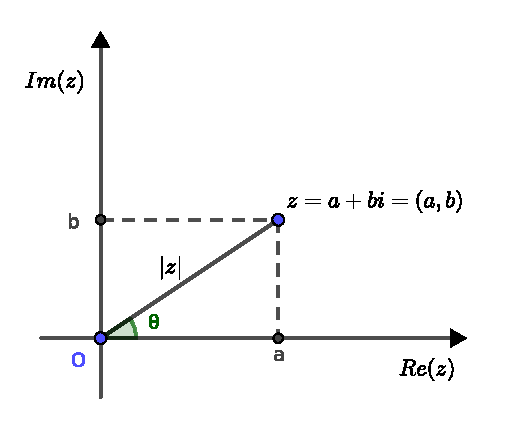
\includegraphics[width=7cm]{plano_complexo.pdf}}
   \caption{Plano complexo}
  \end{figure}

 \item O módulo ou valor absoluto de um número complexo $z= a+bi$ é definido como sendo o número real:
 \[\abs{z}= \sqrt{a^2 + b^2},\]
 o que pode ser deduzido aplicando o teorema de Pitágoras no triângulo retângulo que aparece na figura acima.
 \item No triângulo retângulo formado pelos vértices $O\hat{a}Z$, temos que:
  \begin{align*}
 & \sen(\theta)= \frac{b}{\abs{z}} & & \cos(\theta)= \frac{a}{\abs{z}} &
 \end{align*}
 No qual $\theta$ é o argumento de $z$. Note que $\theta= \arctan \left( \frac{b}{a} \right)$.

 \item O número complexo tem ainda uma representação na forma polar, que é dada por:
 \[z= \abs{z}\cdot (\cos(\theta) + i \sen(\theta))= \abs{z} e^{i \theta} \]

 \end{itemize}
 \end{defi}

 Agora que temos em mãos todas as possíveis apresentações de um número complexo vamos definir as operações dentro deste conjunto.

 \textbf{Soma e subtração:} dados $z_1, z_2 \in \C$ com $z_1= a_1 + b_1i$ e $z_2= a_2 + b_2i$ temos:
 \[z_1 + z_2= (a_1 + a_2) + (b_1 + b_2)i \]
 \[z_1 - z_2= (a_1 - a_2) + (b_1 - b_2)i \]

 \textbf{Multiplicação:} dados $z_1, z_2 \in \C$ com $z_1= a_1 + b_1i$ e $z_2= a_2 + b_2i$ temos:
 \[z_1 \cdot z_2= (a_1 + b_1i) \cdot (a_2 + b_2i)= (a_1a_2 - b_1b_2) + (a_1b_2 + b_1a_2)i \]

 \textbf{Divisão:} dados $z_1, z_2 \in \C$ com $z_1= a_1 + b_1i$ e $z_2= a_2 + b_2i$ temos:
 \[z_1 \div z_2= \frac{a_1 + b_1i}{a_2 + b_2i}= \frac{a_1 + b_1i}{a_2 + b_2i} \cdot \frac{a_2 - b_2i}{a_2 - b_2i} = \frac{(a_1a_2 + b_1b_2) + (b_1a_2 - a_1b_2)i}{a_2^2 + b_2^2} \]

 \textbf{Potência:}
 \begin{align*}
 & i^0= 1 ;& & i^1= i; & & i^2= -1; & & i^3= i \cdot i^2= i \cdot (-1)= -i; & & i^4= i^2 \cdot i^2= (-1)(-1)= 1 .&
 \end{align*}

 Fórmula de Moivre
 \begin{equation}
  z^n= \abs{z}^n[\cos(n \theta) + i \sen(n \theta)]
 \end{equation}

\section{Questões}
\begin{enumerate}
 \item (UFPE/Covest - 2015) A média das alturas de um grupo de funcionários de um escritório é 1,69 m. Quando dois novos funcionários se juntarem ao grupo, a média das alturas permaneceu inalterada. Qual das alternativas a seguir contém possíveis alturas dos dois novos funcionários?
 \begin{enumerate}
 \item 1,65 m e 1,63 m
 \item 1,70 m e 1,68 m
 \item 1,69 m e 1,68 m
 \item 1,79 m e 1,68 m
 \item 1,78 m e 1,68 m
 \end{enumerate}

 \item (UFPE/Covest - 2015) Em um exame, a média dos estudantes de uma turma foi 6,5. A média dos estudantes com nota inferior a 6,5 foi 5,5, e a média dos estudantes com nota igual ou superior a 6,5 foi 7,0. Se a turma era composta por 60 estudantes, quantos estudantes tiveram nota inferior a 6,5?
 \begin{enumerate}
 \item 18
 \item 19
 \item 20
 \item 21
 \item 22
 \end{enumerate}

 \item (UFPE/Covest - 2015) Para ser aprovado em determinada disciplina, um aluno precisa alcançar média maior ou igual a 7,0 nos três exames do semestre, que têm pesos diferentes. Se ele obteve notas respectivas 5,0 e 6,5 nos dois primeiros exames, que têm pesos respectivos 1 e 2, qual a menor nota que ele pode tirar no terceiro exame, que tem peso 3, para ser aprovado na disciplina?
 \begin{enumerate}
 \item 7,5
 \item 8,0
 \item 8,5
 \item 9,0
 \item 9,5
 \end{enumerate}


\end{enumerate}

Gabarito:

\section{Questões}

 \begin{enumerate}
  \item (NC-UFPR - 2017) Considere a seguinte equação com números complexos: $\frac{i - 1}{-2i - 2}$. Assinale a alternativa que apresenta a expressão equivalente a essa equação.
  \begin{enumerate}[a)]
  \item $-0,5 i$.
  \item $0,5$.
  \item $i - 1$.
  \item $2i - 1$.
  \item $i - 2$.
  \end{enumerate}

  \item (IBFC - 2017) Considerando o conjunto numérico que contém as raízes da equação $x^2+1=0$. Os elementos desse conjunto numérico tem a forma $a+bi$, onde $a$ e $b$ são números reais e a unidade imaginária $i$ tem a propriedade $i^2=-1$. As informações referem-se ao conjunto dos números:
  \begin{enumerate}[a)]
  \item Racionais.
  \item Inteiros.
  \item Irracionais.
  \item Complexos.
  \item Naturais.
  \end{enumerate}

  \item (Big Advice - 2017) As afirmações a seguir referem-se aos números complexos

   \begin{enumerate}[I)]
  \item $i^2= -1$.
  \item $i^3= -i$.
  \item $i^5= -i$.
  \end{enumerate}
 A alternativa correta é:
  \begin{enumerate}[a)]
  \item Apenas a I.
  \item Apenas a II.
  \item Apenas a III.
  \item I e II.
  \item I e III.
  \end{enumerate}

  \item (IBFC - 2016) O número complexo que representa o \textbf{conjugado} da soma entre os números complexos $z_1= 3 - 2i$ e $z_2 = 4 + 7i$ é igual a:
  \begin{enumerate}[a)]
  \item $7+5i$.
  \item $-7+5i$.
  \item $-7-5i$.
  \item $7-5i$.
  \end{enumerate}

  \item (IDECAN - 2016) Analise as afirmativas a seguir, marque V para as verdadeiras e F para as falsas.

   \begin{enumerate}[( \ \ )]
  \item $z = (2p + 8) + 3i$ é imaginário puro para $p = -4$.
  \item $z = (k + 2) + (k2 - 4)i$ é real e não nulo se $k = -2$.
  \item Se $z = a + bi$, então $z + \overline{z}$ é sempre real.
  \end{enumerate}
  A sequência está correta em
  \begin{enumerate}[a)]
  \item V, F, V.
  \item V, F, F.
  \item V, V, F.
  \item F, F, V.
  \end{enumerate}

   \item (IFB - 2017) A corrente de um circuito elétrico utiliza em seu cálculo o quociente entre dois números complexos, onde o numerador é a fonte de tensão de uma residência e o denominador é uma carga de impedância. Do resultado deste cálculo utilizam-se as informações do módulo e do argumento para tomar as decisões. Se $a$, $b$ e $c$ são números complexos, tais que $a = -\sqrt{3}+ i$ e $b = 2i$ e $c = \frac{a}{b}$ , o \textbf{módulo} e o \textbf{argumento} do número complexo “$c$” são, respectivamente:

  \begin{enumerate}[a)]
  \item $2$ e $\frac{\pi}{6}$.
  \item $1$ e $\frac{\pi}{3}$.
  \item $2$ e $\frac{\pi}{4}$.
  \item $\frac{1}{2}$ e $\frac{\pi}{3}$.
  \item $1$ e $\frac{\pi}{4}$.
  \end{enumerate}
 \end{enumerate}

 Gabarito: 1 a); 2 d); 3 d); 4 d); 5 a); 6 b).

\chapter{Sistemas De Medida}
%rever questões e colocar em ordem de uso, e unificar a ``cara'' das tabelas.

\section{Medida de tempo}
A unidade padrão para medir tempo de acordo com o Sistema Internacional (SI) é o segundo $(s)$. Cujos múltiplos e submúltiplos são dados pela tabela abaixo:
 \begin{table}[H]
  \centering
  \begin{tabular}{|c|c|c|c|} \hline
  \rowcolor{cinza}
  \multicolumn{1}{|c|}{\textbf{Unid. Fund.}} & \multicolumn{3}{|c|}{\textbf{Múltiplos}} \\ \hline
  segundo & minuto & hora & dia \\ \hline
  s & min & h & d \\ \hline
  $1 s$ & $1 min = 60 s$ & $1 h = 60 min$ & $1 d= 24 h$ \\ \hline
  \end{tabular}
 \end{table}

Além destas unidades de tempo, podemos também relacionar as seguintes unidades:
\begin{table}[H]
\centering
\begin{tabular}{|c|c|} \hline
\rowcolor{cinza}
 \textbf{Unidade} & \textbf{Equivale à} \\ \hline
 Semana & 7 dias \\ \hline
 Quizena & 15 dias \\ \hline
 Mês & 30 dias* \\ \hline
 Bimestre & 2 meses \\ \hline
 Trimestre & 3 meses \\ \hline
 Quadrimestre & 4 meses \\ \hline
 Semestre & 6 meses \\ \hline
 Ano & 12 meses \\ \hline
 Década & 10 anos \\ \hline
 Século & 100 anos \\ \hline
 Milênio & 1000 anos \\ \hline
\end{tabular}
\end{table}

 *O mês comercial utilizado em cálculos financeiros possui por convenção 30 dias.
\newpage

\newpage
\section{Sistema métrico decimal}

\subsection{Medidas de comprimento}
A unidade padrão para medir comprimentos de acordo com o Sistema Internacional (SI) é o metro $(m)$. Cujos múltiplos e submúltiplos são dados pela tabela abaixo:

 \begin{table}[H]
 \centering
 \begin{tabular}{|c|c|c|c|c|c|c|} \hline
 \rowcolor{cinza}
  \multicolumn{3}{|c|}{\textbf{Múltiplos}}
 & \multicolumn{1}{|c|}{\textbf{Unid. Fund.}} & \multicolumn{3}{|c|}{\textbf{Submúltiplos}} \\ \hline
 quilômetro & hectômetro & decâmetro & metro & decímetro & centímetro & milímetro \\ \hline
 $km$ & $hm$ & $dam$ & $m$ & $dm$ & $cm$ & $mm$ \\ \hline
 $1000 m$ & $100 m$  & $10 m$ & $1 m$ & $0,1 m$ & $0,01 m$ & $0,001 m$ \\ \hline
 $10^3 m$ & $10^2 m$ & $10^1 m$ & $1 m$ & $10^{-1} m$ & $10^{-2} m$ & $10^{-3} m$ \\ \hline
 \end{tabular}
 \end{table}

 Existem outras unidades de medida mas que não pertencem ao sistema métrico decimal. Vejamos as relações entre algumas dessas unidades e as do sistema métrico decimal:

1 polegada = 25,4 milímetros

1 milha = 1 609 metros

1 légua = 5 555 metros

1 pé = 30 centímetros

Obs: valores aproximados.



\subsection{Medidas de superfície}
A unidade padrão para medir superfície de acordo com o Sistema Internacional (SI) é o metro quadrado $(m^2)$. Cujos múltiplos e submúltiplos são dados pela tabela abaixo:

 \begin{table}[H]
 \centering
 \begin{tabular}{|c|c|c|c|c|c|c|} \hline
 \rowcolor{cinza}
  \multicolumn{3}{|c|}{\textbf{Múltiplos}}
 & \multicolumn{1}{|c|}{\textbf{Unid. Fund.}} & \multicolumn{3}{|c|}{\textbf{Submúltiplos}} \\
 \hline
 $km^2$ & $hm^2$ & $dam^2$ & $m^2$ & $dm^2$ & $cm^2$ & $mm^2$ \\
 \hline
 $1000 000 m^2$ & $10 000 m^2$ & $100 m^2$ & $1 m^2$ & $0,01 m^2$ & $0,0001 m^2$ & $0,000001 m^2$ \\ \hline
 $10^6 m^2$ & $10^4 m^2$ & $10^2 m^2$ & $1 m^2$ & $10^{-2} m^2$ & $10^{-4} m^2$ & $10^{-6} m^2$ \\ \hline
 \end{tabular}
 \end{table}

 Quando queremos medir grandes porções de terra (como sítios, fazendas etc.) usamos uma unidade agrária chamada hectare $(ha)$.

O hectare é a medida de superfície de um quadrado de $100 m$ de lado.

$1$ hectare $(ha)$ = $1 hm^2$ = $10 000 m^2$

Em alguns estados do Brasil, utiliza-se também uma unidade não legal chamada alqueire.

    1 alqueire mineiro é equivalente a $48 400 m^2$.

    1 alqueire paulista é equivalente a $24 200 m^2$.



\subsection{Medidas de volume}
A unidade padrão para medir volume de acordo com o Sistema Internacional (SI) é o metro cúbico $(m^3)$. Cujos múltiplos e submúltiplos são dados pela tabela abaixo:

 \begin{table}[H]
 \centering
 \begin{tabular}{|c|c|c|c|c|c|c|} \hline
 \rowcolor{cinza}
  \multicolumn{3}{|c|}{\textbf{Múltiplos}}
 & \multicolumn{1}{|c|}{\textbf{Unid. Fund.}} & \multicolumn{3}{|c|}{\textbf{Submúltiplos}} \\
 \hline
 $km^3$ & $hm^3$ & $dam^3$ & $m^3$ & $dm^3$ & $cm^3$ & $mm^3$ \\
 \hline
 $1000 000 000 m^3$ & $1000 000 m^3$ & $1000 m^3$ & $1 m^3$ & $0,001 m^3$ & $0,000001 m^3$ & $0,000000001 m^3$ \\ \hline
 $10^9 m^3$ & $10^6 m^3$ & $10^3 m^3$ & $1 m^3$ & $10^{-3} m^3$ & $10^{-6} m^3$ & $10^{-9} m^3$ \\ \hline
 \end{tabular}
\end{table}

\subsection{Medidas de capacidade}
A unidade padrão para medir capacidade de um sólido de acordo com o Sistema Internacional (SI) é o litro $(l)$.

De acordo com o Comitê Internacional de Pesos e Medidas, o litro é, aproximadamente, o volume equivalente a um decímetro cúbico, ou seja:

$1$ litro= $1,000027 dm^3$

Porém, na prática, definimos:
$1$ litro = $1 dm^3$.

Cujos múltiplos e submúltiplos são dados pela tabela abaixo:

 \begin{table}[H]
 \centering
 \begin{tabular}{|c|c|c|c|c|c|} \hline
 \rowcolor{cinza}
  \multicolumn{2}{|c|}{\textbf{Múltiplos}}
 & \multicolumn{1}{|c|}{\textbf{Unid. Fund.}} & \multicolumn{3}{|c|}{\textbf{Submúltiplos}} \\
 \hline
 hectolitro & decalitro & litro & decilitro & centilitro & mililitro \\
 \hline
 $hl$ & $dal$ & $l$ & $dl$ & $cl$ & $ml$ \\ \hline
 $100 l$ & $10 l$ & $1 l$ & $0,1 l$ & $0,01 l$ & $0,001 l$\\ \hline
 $10^2 l$ & $10^1 l$ & $1 l$ & $10^{-1} l$ & $10^{-2} l$ & $10^{-3} l$\\ \hline
 \end{tabular}
\end{table}

Obs: Não é usado nem consta da lei o quilolitro.



\section{Sistema monetário brasileiro}
O sistema monetário de um país é composto por regras e bancos comerciais e estatais responsáveis pela circulação da moeda. No Brasil a moeda vigente é o Real e o órgão responsável pela administração e produção de cédulas e moedas é o Banco Central.

Historicamente o Brasil teve as seguintes moedas:

 \begin{table}[H]
 \centering
 \begin{tabular}{|c|c|c|c|} \hline
 \rowcolor{cinza}
 \multicolumn{4}{|c|}{\textbf{Unidades do sistema monetário Brasileiro}} \\
 \hline
 \textbf{Unidade monetária} & \textbf{Período de vigência} & \textbf{Símbolo} & \textbf{Correspondência} \\
\hline
Real (plural= Réis) & Período colonial até 07/10/1833 & R & R 1\$2000= 1/8 ouro de 22K \\
\hline
Mil Réis & 08/10/1833 a 31/10/1942 & R\$ & Rs 2\$500= 1/8 de ouro de 22K \\
\hline
Cruzeiro & 01/11/1942 a 30/11/1964 & Cr\$ & Cr\$ 1,00= Rs 1\$000 \\
\hline
Cruzeiro & 01/12/1964 a 12/02/1967 & Cr\$ & Cr\$ 1= Cr\$ 1,00 \\
\hline
Cruzeiro Novo & 13/02/1967 a 14/05/1970 & NCr\$ & Cz\$ 1,00= Cr\$ 1.000 \\
\hline
Cruzado Novo & 16/01/1989 a 15/03/1990 & NCz\$ & NCz\$= Cz\$ 1.000,00 \\
\hline
Cruzeiro & 16/03/1990 a 31/07/1993 & Cr\$ & Cr\$ 1,00= NCz\$ 1,00 \\
\hline
Cruzeiro Real & 01/08/1993 a 30/06/1994 & CR\$ & CR\$ 1,00= Cr\$ 1.000,00 \\
\hline
Real (plural= Reais) & A partir de 01/07/1994 & R\$ & R\$ 1,00= CR\$2.750,00 \\
\hline

\end{tabular}
\caption{Moedas Brasileiras.}
\end{table}


\section{Medida de massa}
A unidade padrão para medir massa de um sólido de acordo com o Sistema Internacional (SI) é o quilograma $(kg)$. Cujo submúltiplo mais utilizado é o grama $(g)$, mas este não é o único. Vejamos na tabela abaixo todos os múltiplos e submúltiplos do quilograma:

 \begin{table}[H]
 \centering
 \begin{tabular}{|c|c|c|c|c|c|c|} \hline
 \rowcolor{cinza}
  \multicolumn{3}{|c|}{\textbf{Múltiplos}}
 & \multicolumn{1}{|c|}{\textbf{Unid. Fund.}} & \multicolumn{3}{|c|}{\textbf{Submúltiplos}} \\
 \hline
 tonelada & quilograma & decagrama & grama & decigrama & centigrama & miligrama \\
 \hline
 $t$ & $kg$ & $dag$ & $g$ & $dg$ & $cg$ & $mg$ \\ \hline
 $1000000 g$ & $1000 g$ & $10 g$ & $1 g$ & $0,1 g$ & $0,01 g$ & $0,001 g$ \\ \hline
 $10^6 g$ & $10^3 g$ & $10^1 g$ & $1 g$ & $10^{-1} g$ & $10^{-2} g$ & $10^{-3} g$ \\ \hline
 \end{tabular}
\end{table}

\chapter{Lógica}

De acordo com (www.dicio.com.br); uma sentença é uma construção sintática com sentido completo, composta por uma ou mais palavras; frase. E de acordo com (michaelis.uol.com.br) uma sentença é uma frase, uma oração ou qualquer declaração sem levar em conta sua falsidade ou veracidade; proposição.

No Português, as sentenças são classificadas de diversas formas. Exemplo:
\begin{itemize}
 \item Interrogativas: ``Vai chover hoje?''
 \item Imperativas: ``Leve guarda-chuva!''
 \item Declarativas: ``Eu estou estudando matemática.''
\end{itemize}

As sentenças que são objetos de estudo na \emph{lógica proposicional} ou \emph{lógica sentencial} são as sentenças declarativas, que podem ser classificadas como verdadeiras ou falsas, mas não como verdadeira e falsa simultaneamente. Como por exemplo:

\begin{enumerate}
 \item A lógica é uma ramo do conhecimento.
 \item A UDESC é uma Universidade Estadual.
 \item A matemática é uma ciência.
 \item Os gatos não são animais.
\end{enumerate}


Chamamos estas sentenças de \textbf{proposição}.

As proposições são ditas \emph{simples} quando não possuem nenhum dos conectivos lógicos: ``não'', ``e'', ``ou'', ``se $\cdots$ então'', ``se e somente se''. Por exemplo:
\begin{center}
Santa Catarina é um estado.
\end{center}
Elas são consideradas as unidades básicas do discurso. A partir da combinação destas por intermédio dos conectivos lógicos: ``não'', ``e'', ``ou'', ``se $\cdots$ então'', ``se e somente se'', constroem-se sentenças mais complexas chamadas de \emph{proposições compostas}. Por exemplo:
\begin{center}
A UFSC é uma Universidade Federal e gratuita.
\end{center}

 No contexto da Lógica as proposições serão denotadas por $P$, $Q$, $R$, $S$, $P_1$, $Q_1$, $R_1$, $S_1$, e assim por diante. Assim por vezes ao invés de escrever a proposição iremos nos referir a ela através de um destes símbolos. Principalmente quando estivermos verificando o valor verdade de proposições compostas, afinal como veremos a seguir, nesta situação estaremos preocupados com o conectivo lógico e com os valores verdade de cada uma das proposições simples que a compõem.

 Antes de nos preocuparmos com os valores verdade das proposições compostas, vamos entender melhor estas proposições.

 A primeira coisa que precisamos saber é que as proposições compostas recebem nomes específicos de acordo com o tipo de conectivo lógico que possuem. Desta forma dadas as proposições $P, Q, R$ diremos que:

 \begin{itemize}
  \item $P$ é uma \textbf{negação} se $P$ for da forma ``não vale $Q$''.
  \item $P$ é uma \textbf{conjunção} se $P$ for da forma ``$Q$ e $R$''.
  \item $P$ é uma \textbf{disjunção} se $P$ for da forma ``$Q$ ou $R$''.
  \item $P$ é uma \textbf{implicação} se $P$ for da forma ``Se $Q$ então $R$''.
  \item $P$ é uma \textbf{bi-implicação} se $P$ for da forma ``$Q$ se e somente se $R$''.
 \end{itemize}

 Vejamos alguns exemplos de cada um destes tipos de proposição composta, para entender como a partir de proposições simples podemos chegar em uma proposição composta, e como a partir de uma proposição composta identificamos quais são as proposições simples que a compõem.

 \begin{itemize}
  \item \textbf{Negação:} Neste exemplos consideremos como dada a proposição $Q$, e vejamos como fica sua negação.

  \begin{exem} \label{(Neg. 1)}
    $Q:$ A Copa do Mundo FIFA de 2014 foi realizada no Brasil. (V) \\
    $\sim Q= P:$ A Copa do Mundo FIFA de 2014 não foi realizada no Brasil. (F)
  \end{exem}

 \begin{exem} \label{(Neg. 2)}
   $Q:$ O gato não pertence a família dos felinos. (F)\\
   $\sim Q= P:$ O gato pertence a família dos felinos. (V)
 \end{exem}

 \begin{exem} \label{(Neg. 3)}
   $Q:$ O escorpião é um inseto. (F)\\
   $\sim Q= P:$ O escorpião não é um inseto. (V)
 \end{exem}


 \item \textbf{Conjunção}


  \begin{exem} \label{(E 1)}
 Considere a seguinte proposição composta $P$.

 $P:$ O termo coruja é a designação comum das aves estrigiformes, das famílias dos titonídeos e estrigídeos. (V)

 Note que a proposição $P$ é a conjunção das seguintes proposições simples:\\
 $Q:$ O termo coruja é a designação comum das aves estrigiformes, da família dos titonídeos. \\
 $R:$ O termo coruja é a designação comum das aves estrigiformes, da família dos estrigídeos.
 \end{exem}

 \begin{exem} \label{(E 2)}
 Façamos agora o processo inverso, dadas as proposições simples $Q$ e $R$:

 $Q:$ O gato angorá é uma raça de gato doméstico. (V)\\
 $R:$ O gato angorá surgiu na região de Ancara, na Turquia. (V)

 Obtemos a seguinte proposição composta:\\
 $P= (Q$ e $R):$ O gato angorá é uma raça de gato doméstico que surgiu na região de Ancara, na Turquia.

 Apesar da conjunção $e$ não aparecer explicitamente na proposição $P$, temos que $P= (Q$ e $R)$.
 \end{exem}

 \begin{exem} \label{(E 3)}
 Dadas as proposições simples $Q$ e $R$:

 $Q:$  Charles Darwin estudou a evolução das espécies.(V)\\
 $R:$  O reality show Big Brother Brasil teve sua primeira edição no ano 2000. (F)

 Obtemos a seguinte proposição composta:\\
 $P= (Q$ e $R):$ Charles Darwin estudou a evolução das espécies e o reality show Big Brother Brasil teve sua primeira edição no ano 2000.
 \end{exem}

 \begin{exem} \label{(E 4)}
 Dadas as proposições simples $Q$ e $R$:

 $Q:$  O reality show A Fazenda é um show de talentos de culinária brasileiro. (F)\\
 $R:$  O reality show MasterChef Brasil mostra os participantes em uma fazenda lidando com tarefas típicas do meio rural.(F)

 Obtemos a seguinte proposição composta:\\
 $P= (Q$ e $R):$ O reality show A Fazenda é um show de talentos de culinária brasileiro e o reality show MasterChef Brasil mostra os participantes em uma fazenda lidando com tarefas típicas do meio rural.
 \end{exem}


 \item \textbf{Disjunção}

  \begin{exem} \label{(Ou 1)}
 Considere a seguinte proposição:

 $P:$ A ansiedade pode causar sintomas físicos, como ritmo cardíaco acelerado ou tremores. (V)

 Observe que $P$ é a disjunção das seguintes proposições $Q$ e $R$.

 $Q:$ A ansiedade pode causar sintomas físicos, como ritmo cardíaco acelerado. \\
 $R:$ A ansiedade pode causar sintomas físicos, como tremores.
 \end{exem}

 \begin{exem} \label{(Ou 2)}
 Dadas as seguintes proposições simples $Q$ e $R$:

 $Q:$ O Império Inca foi um Estado criado pela civilização inca. (V) \\
 $R:$ Roma Antiga foi uma civilização que se desenvolveu a partir da cidade-estado de Roma. (V)

 Podemos obter a seguinte proposição composta $P$:

 $P= (Q$ ou $R):$ O Império Inca foi um Estado criado pela civilização inca, ou, Roma Antiga foi uma civilização que se desenvolveu a partir da cidade-estado de Roma.
 \end{exem}

 \begin{exem} \label{(Ou 3)}
 Analogamente, dadas as seguintes proposições simples $Q$ e $R$:

 $Q:$ O Aquecimento global é o processo de aumento da temperatura média dos oceanos e da atmosfera da Terra. (V) \\
 $R:$ A massa e o peso são a mesma unidade de medida. (F)

 Podemos obter a seguinte proposição composta $P$:

 $P= (Q$ ou $R):$ O Aquecimento global é o processo de aumento da temperatura média dos oceanos e da atmosfera da Terra, ou, a massa e o peso são a mesma unidade de medida.
 \end{exem}


 \item \textbf{Implicação}

 Vamos agora a exemplos nos quais dadas as proposições simples $Q$ e $R$ construímos a proposição composta $P$ dada por: Se $Q$ então $R$.

  \begin{exem} \label{(Se 1)}
 $Q:$ Estou no planeta Terra. (V) \\
 $R:$ Estou sofrendo uma ação da força gravitacional de $9,8 m/s^2$.(V) \\
 $P=$ Se $Q$ então $R$: Se estou no planeta Terra então estou sofrendo uma ação da força gravitacional de $9,8 m/s^2$.

 Neste caso a implicação recebe também o nome de \textbf{condicional}, pois a proposição $Q$ é uma condição para que a proposição $R$ ocorra.\end{exem}

 \begin{exem} \label{(Se 2)}
 $Q:$ O Hidrogênio é um elemento químico de símbolo H. (V) \\
 $R:$ A Oceania é um país. (F) \\
 $P=$ Se $Q$ então $R$: Se o Hidrogênio é um elemento químico de símbolo H então a Oceania é um país.
 \end{exem}

 \begin{exem} \label{(Se 3)}
 $Q:$ Os anéis de Saturno são um sistema de anéis que circunda o planeta Terra. (F) \\
 $R:$ Isaac Newton foi um cientista inglês, considerado o pai da Mecânica Clássica. (V) \\
 $P=$ Se $Q$ então $R$: Se os anéis de Saturno são um sistema de anéis que circunda o planeta Terra então Isaac Newton foi um cientista inglês, considerado o pai da Mecânica Clássica.
 \end{exem}

 \begin{exem} \label{(Se 4)}
 $Q:$ A atmosfera terrestre é uma camada de rochas que envolve a Terra. (F) \\
 $R:$ Stephen William Hawking é um biólogo. (F) \\
 $P=$ Se $Q$ então $R$: Se a atmosfera terrestre é uma camada de rochas que envolve a Terra então Stephen William Hawking é um biólogo.
 \end{exem}


 Observe que para se ter uma proposição composta do tipo implicação não é obrigatório que as proposições simples que a compõem tenham relação, quando isso ocorre a implicação recebe o nome de condicional.

 \item \textbf{Bi-implicação}

 Dadas as proposições simples $Q$ e $R$ abaixo, podemos construir a proposição composta $P=$ $Q$ e somente se $R$.

  \begin{exem} \label{(Def 1)}
  $Q:$ Uma mulher experimenta amor romântico ou atração sexual por outra mulher.\\
 $R:$ A mulher é lésbica. \\
 $P=$ $Q$ e somente se $R$: Uma mulher experimenta amor romântico ou atração sexual por outra mulher e somente se ela é lésbica.
 \end{exem}

 \begin{exem} \label{(Def 2)}
 $Q:$ O sistema operacional utiliza o núcleo Linux. \\
 $R:$ O sistema operacional é Linux. \\
 $P=$ $Q$ e somente se $R$: Se o sistema operacional utiliza o núcleo Linux e somente se ele é Linux.
 \end{exem}

 Note que nestes dois exemplos, a bi-implicação é utilizada para expressar os significados dos termos lésbica e Linux, respectivamente. Porém podemos construir uma bi-implicação e analisar seu valor verdade sem que as proposições simples que a compõem tenham relação. Vejamos uns exemplos de bi-implicações nas quais as proposições simples não possuem relação.


 \begin{exem} \label{(Sse 1)}
 Consideremos as seguintes proposições $Q$ e $R$:\\
 $Q:$ A berinjela é uma fruta. (V) \\
 $R:$ Barroco é um estilo artístico que floresceu inicialmente na Itália. (V)

 A partir destas proposições obtemos:\\
 $P=$ $Q$ e somente se $R$: A berinjela é uma fruta se e somente se o Barroco é um estilo artístico que floresceu inicialmente na Itália.
 \end{exem}

 \begin{exem} \label{(Sse 2)}
 Consideremos as seguintes proposições $Q$ e $R$:\\
 $Q:$ A meiose é o tipo de divisão celular que leva à redução do número de cromossomos para metade. (V) \\
 $R:$ Macapá é a capital do Acre. (F)

 A partir destas proposições obtemos:\\
 $P=$ $Q$ e somente se $R$:  A meiose é o tipo de divisão celular que leva à redução do número de cromossomos para metade se e somente se Macapá é a capital do Acre.
 \end{exem}

 \begin{exem} \label{(Sse 3)}
 Consideremos as seguintes proposições $Q$ e $R$:\\
 $Q:$ A Primeira Guerra Mundial começou em 1913.  (F) \\
 $R:$ A Segunda Guerra Mundial começou em 1940. (F)

 A partir destas proposições obtemos:\\
 $P=$ $Q$ e somente se $R$:  A Primeira Guerra Mundial começou em 1913 se e somente se a Segunda Guerra Mundial começou em 1940.
 \end{exem}

 \end{itemize}

 Quando vamos estudar o valor verdade de proposições compostas precisamos lembrar que devemos nos preocupar apenas com os valores verdade das proposições simples que as compõem, por isso representamos as proposições simples por letras e os conectivos lógicos pelos seguintes sinais:

 \begin{table}[H]
  \centering
 \begin{tabular}{|c|c|} \hline
 \rowcolor{verde}
 \textbf{Conectivos Lógicos} & \textbf{Símbolos} \\ \hline
 não $\cdots$ & $\sim$ ou $\neg$ \\ \hline
 $\cdots$ e $\cdots$ &  $\land$ \\ \hline
 $\cdots$ ou $\cdots$ &  $\lor$ \text{ ou } $\veebar$ \\ \hline
 se $\cdots$ então $\cdots$ &  $\rightarrow$ \\ \hline
 $\cdots$ se e somente se $\cdots$ & $\leftrightarrow$ \\ \hline
 \end{tabular}
 \caption{Conectivos lógicos - Símbolos}
\end{table}


 Assim, dadas as proposições $Q$ e $R$, podemos representar simbolicamente a proposição $P$ composta por $Q$ e $R$ de acordo com a tabela abaixo:

 \begin{table}[H]
 \centering
 \begin{tabular}{|c|c|} \hline
 \rowcolor{verde}
 \textbf{Proposições compostas} & \textbf{Símbolos} \\ \hline
 $P:$ a negação de $Q$ & $\sim Q$ \\ \hline
 $P:$ a conjunção de $Q$ e $R$ &  $Q \land R$ \\ \hline
 $P:$ a disjunção inclusiva de $Q$ e $R$ &  $Q \lor R$ \\ \hline
 $P:$ a disjunção exclusiva de $Q$ e $R$ &  $Q \veebar R$ \\ \hline
 $P:$ se $Q$ então $R$ &  $Q \rightarrow R$ \\ \hline
 $P:$ $Q$ se e somente se $R$ & $Q \leftrightarrow R$ \\ \hline
 \end{tabular}
 \caption{Proposições compostas - Símbolos}
\end{table}

Como as proposições compostas podem possuir mais de um conectivo lógico, assim como as expressões matemáticas podem possuir mais de uma operação, é aqui também necessário definir um ordem de precedência dos conectivos proposicionais. Esta ordem de precedência é a seguinte:
\begin{itemize}
 \item Maior precedência: $\sim$ ou $\neg$;
 \item Precedência intermediária: $ \rightarrow $ ou $ \leftrightarrow $;
 \item Menor precedência: $\land$, $\lor$ ou $\veebar$.
\end{itemize}

 Estamos agora aptos a começar o estudo do valor verdade de uma proposição composta $P$. Como já comentado o valor verdade de uma proposição composta independe do conteúdo de suas proposições, tendo como base somente os valores verdade de cada uma das proposições simples que a compõem e o conectivo lógico que as relaciona. De posse destas informações a ferramenta que nos permite decidir se $P$ é verdadeira ou falsa é a tabela verdade de seu conectivo lógico. Na próxima seção apresentamos as tabelas verdade de cada uma das proposições e como utilizá-las.

\section{Tabelas verdade básicas}

 Dadas duas proposições quaisquer $Q$ e $R$ e um dos conectivos lógicos $\{\neg, \land, \lor, \veebar, \rightarrow, \leftrightarrow \}$, a tabela verdade deste conectivo, é a ferramenta que nos diz quais são todos os possíveis valores verdades da proposição composta por $Q$ e $R$ através deste conectivo, considerando todas as possíveis combinações de valores verdade destas proposições.

 Vamos começar estudando a Negação.

 A tabela abaixo representa os possíveis valores verdade de $P$ e de sua negação ($\neg P$). Através dela concluímos também a \textbf{Lei da dupla negação}:

  \[\destaque{P \leftrightarrow \neg(\neg P)}\]

 \begin{table}[H]
 \centering
 \begin{tabular}{|c|c|c|c|} \hline
 \rowcolor{cinza}
 $P$ & $\neg P$ & $\neg (\neg P)$ & $ P \leftrightarrow \neg (\neg P)$\\ \hline
 V & F & V & V \\ \hline
 F & V & F & V \\ \hline
 \end{tabular}
 \caption{Negação}
\end{table}

 Já vimos alguns exemplos simples de negação, e seus valores verdade. Vamos agora à um exemplo mais elaborado do uso da negação, no qual utilizaremos o fato da dupla negação $\neg(\neg P)$ ser equivalente a afirmação $P$.

 \begin{exem}
 $Q:$ A cannabis não é ilegal no Brasil.\\
 $\sim Q:$ A cannabis não é legalizada no Brasil.

 Lembremos aqui que:
   \[\text{ilegal= não é legalizada}\]
 logo,
   \[\text{não é ilegal= não, não é legalizada}\]
 como $P \leftrightarrow \neg(\neg P)$ sendo, $P:$ é legalizada, obtemos que:
   \[\text{não é ilegal= não, não é legalizada= é legalizada.}\]
 Portanto,
    \[\sim P:\text{não é legalizada.}\]

    \fim
 \end{exem}


 Tabela verdade da conjunção de $Q$ com $R$ ($(Q \land R)= (Q \text{ e } R)$):

 \begin{table}[H]
 \centering
 \begin{tabular}{|c|c|c|} \hline
 \rowcolor{cinza}
 $Q$ & $R$ & $Q \land R$ \\ \hline
 V & V & V  \\ \hline
 V & F & F  \\ \hline
 F & V & F  \\ \hline
 F & F & F \\ \hline
 \end{tabular}
 \caption{Conjunção - e}
\end{table}

\begin{exem}
 Voltamos para o exemplo \ref{(E 1)}, neste exemplo a proposição $P$ é uma proposição composta com conectivo lógico $e$, e sabemos que $P$ é verdadeira, então pela 1ª linha da tabela verdade acima percebemos que a única forma desta proposição composta ser verdade é que cada uma de suas proposições simples sejam verdadeiras, portanto as proposições $Q$ e $R$ são verdadeiras.

 No exemplo \ref{(E 2)} temos que as proposições $Q$ e $R$ são verdadeiras, portanto também pela 1ª linha da tabela da conjunção concluímos que a proposição composta $P= Q \land R$ é verdadeira.

 Já nos exemplos \ref{(E 3)} e \ref{(E 4)} ao menos uma das proposições $Q$, $R$ são falsas, portanto da tabela acima concluímos que a proposição $P$ é falsa.
\end{exem}


 Tabela verdade da disjunção inclusiva de $P$ com $Q$ ($(P \lor Q)= (P \text{ ou } Q)$):
 \begin{table}[H]
 \centering
 \begin{tabular}{|c|c|c|} \hline
 \rowcolor{cinza}
 $P$ & $Q$ & $P \lor Q$ \\ \hline
 V & V & V \\ \hline
 V & F & V \\ \hline
 F & V & V \\ \hline
 F & F & F \\ \hline
 \end{tabular}
 \caption{Disjunção inclusiva - ou}
\end{table}

 \begin{exem}
  Voltemos aos exemplos \ref{(Ou 1)} , \ref{(Ou 2)} , \ref{(Ou 3)} .

  No exemplo \ref{(Ou 1)} é dada um proposição composta $P$ verdadeira, então pela tabela verdade acima, temos três possibilidades:
  \begin{itemize}
   \item $Q$: V e $R$: V
   \item $Q$: V e $R$: F
   \item $Q$: F e $R$: V
  \end{itemize}
  logo, na podemos afirmar sobre os valores verdade de $Q$ e $R$.

  No exemplo \ref{(Ou 2)}, como $Q$ e $R$ são verdadeiras, pela 1ª linha da tabela concluímos que $P$ é verdadeira. E no exemplo \ref{(Ou 3)} como somente $R$ é falsa, pela 2ª linha da tabela temos que $P$ é verdadeira.

 \end{exem}

 Tabela verdade da disjunção exclusiva de $P$ com $Q$ ($(P \veebar Q)= (P \text{ ou } Q)$):
 \begin{table}[H]
 \centering
 \begin{tabular}{|c|c|c|} \hline
 \rowcolor{cinza}
 $P$ & $Q$ & $P \veebar Q$ \\ \hline
 V & V & F \\ \hline
 V & F & V \\ \hline
 F & V & V \\ \hline
 F & F & F \\ \hline
 \end{tabular}
 \caption{Disjunção exclusiva - ou}
\end{table}


 Tabela verdade da implicação de $P$ em $Q$ ($P \rightarrow Q $):
 \begin{table}[H]
 \centering
 \begin{tabular}{|c|c|c|} \hline
 \rowcolor{cinza}
 $P$ & $Q$ & $P \rightarrow Q$ \\ \hline
 V & V & V \\ \hline
 V & F & F \\ \hline
 F & V & V \\ \hline
 F & F & V \\ \hline
 \end{tabular}
 \caption{Implicação - $(\rightarrow$)}
\end{table}

 \begin{exem}
  Vamos agora analisar aos exemplos \ref{(Se 1)} , \ref{(Se 2)} , \ref{(Se 3)} , \ref{(Se 4)}.

  De posse da tabela verdade da implicação concluímos que dos exemplos citados acima o único que gerou uma proposição composta $P$ cujo valor verdade é falso é o exemplo \ref{(Se 2)}. Já nos exemplos \ref{(Se 1)} , \ref{(Se 3)} e \ref{(Se 4)} os valores verdade de suas proposições simples estão presentes, respectivamente, nas linhas 1, 3 e 4 da tabela verdade, o que nos leva a concluir que a proposição composta $P$ é verdadeira nestes casos.

  \end{exem}

  Tabela verdade da bi-implicação de $P$ com $Q$ ($P \leftrightarrow Q $):
 \begin{table}[H]
 \centering
 \begin{tabular}{|c|c|c|} \hline
 \rowcolor{cinza}
 $P$ & $Q$ & $P \leftrightarrow Q$ \\ \hline
 V & V & V \\ \hline
 V & F & F \\ \hline
 F & V & F \\ \hline
 F & F & V \\ \hline
 \end{tabular}
 \caption{Bi - implicação - ($\leftrightarrow$)}
\end{table}

 \begin{exem}
  Para compreender o uso da tabela verdade da Bi-implicação, voltemos aos exemplos \ref{(Sse 1)} , \ref{(Sse 2)} , \ref{(Sse 3)} .

  O exemplo \ref{(Sse 1)}, possui seus valores verdade presentes na 1ª linha da tabela, portanto neste caso concluímos que a proposição $P$ é verdadeira.

  As linhas 2 e 3 da tabela podem ser aplicadas ao exemplo \ref{(Sse 2)} , o que nos leva a conclusão que neste caso $P$ é falsa.

  Já no exemplo \ref{(Sse 3)} , apesar de $Q$ e $R$ serem ambas falsas a tabela nos garante que $P$ é verdadeira.
 \end{exem}


 \section{Resultados importantes}

 \colorbox{azul}{
 \begin{minipage}{0.9\linewidth}
 \begin{center}
 Uma proposição $P$ é dita ser uma \textbf{Tautologia} quando seu único valor verdade possível é o \emph{verdadeiro}.
 \end{center}
 \end{minipage}}


 \begin{exem}
  Dada uma proposição $P$ qualquer a proposição composta $Q= P \lor \neg P$ é uma tautologia como pode ser observado pela sua tabela verdade abaixo:
  \begin{table}[H]
  \centering
  \begin{tabular}{|c|c|c|} \hline
  \rowcolor{cinza}
  $P$ & $\neg P$ & $P \lor \neg P$ \\ \hline
  V & F & V \\ \hline
  F & V & V \\ \hline
  \end{tabular}
  \end{table}
\end{exem}

 \colorbox{amarelo}{
 \begin{minipage}{14cm}
 \begin{center}
 O fato de a fórmula $P \lor \neg P$ ser uma tautologia está relacionado ao \textbf{princípio do terceiro-excluído}: dada uma proposição e sua negação, pelo menos uma delas é verdadeira ($P \lor \neg P$).
 \end{center}
 \end{minipage}}

 \vskip0.3cm

 \colorbox{azul}{
 \begin{minipage}{14cm}
 \begin{center}
 Uma proposição $P$ é dita ser uma \textbf{Contradição} quando seu único valor verdade possível é o \emph{falso}.
 \end{center}
 \end{minipage}}

 \vskip0.3cm

\begin{exem}
  Dada uma proposição $P$ qualquer a proposição composta $Q= P \land \neg P$ é uma contradição como pode ser observado pela sua tabela verdade abaixo:
  \begin{table}[H]
  \centering
  \begin{tabular}{|c|c|c|} \hline
  \rowcolor{cinza}
  $P$ & $\neg P$ & $P \land \neg P$ \\ \hline
  V & F & F \\ \hline
  F & V & F \\ \hline
  \end{tabular}
  \end{table}
\end{exem}

 Este exemplo mostra que a proposição $Q= P \land \neg P$ é uma contradição.

 \vskip0.3cm

 \colorbox{amarelo}{
 \begin{minipage}{14cm}
 \begin{center}
 Se a proposição $Q= P \land \neg P$ é uma contradição, então $\neg Q= \neg ( P \land \neg P)$ é uma tautologia. Isto está relacionado com o \textbf{princípio da não-contradição}: dada uma proposição e sua negação, pelo menos uma delas é falsa ($\neg(P \land \neg P)$).
 \end{center}
 \end{minipage}}

 \vskip0.3cm

 \colorbox{azul}{
 \begin{minipage}{14cm}
 \begin{center}
 \textbf{Leis de De Morgan}

 A primeira Lei de De Morgan é definida pela fórmula
 \[\neg(P \land Q) \leftrightarrow (\neg P \lor \neg Q)\]
 que é uma tautologia.
 \end{center}
 \end{minipage}}

 \vskip0.3cm

 Essa lei define uma regra para a distribuição do conectivo $\neg$ em uma conjunção. Observe que o conectivo $\land$ se transforma no conectivo $\lor$. A tabela verdade abaixo demonstra a veracidade desta lei:

 \begin{table}[H]
 \centering
 \begin{tabular}{|c|c|c|c|c|c|c|c|} \hline
 \rowcolor{cinza}
 $P$ & $\neg P$ & $Q$ & $\neg Q$ & $P \land Q$ & $\neg (P \land Q)$ & $\neg P \lor \neg Q$ & $\neg(P \land Q) \leftrightarrow (\neg P \lor \neg Q)$ \\ \hline
 V & F & V & F & V & F & F & V \\ \hline
 V & F & F & V & F & V & V & V \\ \hline
 F & V & V & F & F & V & V & V \\ \hline
 F & V & F & V & F & V & V & V \\ \hline
 \end{tabular}
 \end{table}

 \colorbox{azul}{
 \begin{minipage}{14cm}
 \begin{center}
 A segunda Lei de De Morgan é definida pela fórmula
 \[\neg(P \lor Q) \leftrightarrow (\neg P \land \neg Q)\]
 que também é uma tautologia.
 \end{center}
 \end{minipage}}

 \vskip0.3cm

 Essa lei define uma regra para a distribuição do conectivo $\neg$ em uma disjunção. Observe que o conectivo $\lor$ se transforma no conectivo $\land$. A tabela verdade abaixo demonstra a veracidade desta lei:

 \begin{table}[H]
 \centering
 \begin{tabular}{|c|c|c|c|c|c|c|c|} \hline
 \rowcolor{cinza}
 $P$ & $\neg P$ & $Q$ & $\neg Q$ & $P \lor Q$ & $\neg (P \lor Q)$ & $\neg P \land \neg Q$ & $\neg(P \lor Q) \leftrightarrow (\neg P \land \neg Q)$ \\ \hline
 V & F & V & F & V & F & F & V \\ \hline
 V & F & F & V & V & F & F & V \\ \hline
 F & V & V & F & V & F & F & V \\ \hline
 F & V & F & V & F & V & V & V \\ \hline
 \end{tabular}
\end{table}

 \vskip0.3cm

 Ainda da seção de negações é importante ressaltar a negação de uma implicação:

  \colorbox{azul}{
 \begin{minipage}{14cm}
 \begin{center}
 \textbf{Negação da implicação}

 \[\neg (P \rightarrow Q) = P \land \neg Q\]

 \end{center}
 \end{minipage}}

 \vskip0.3cm

 \colorbox{azul}{
 \begin{minipage}{14cm}
 \begin{center}
 \textbf{Lei da contraposição}

 A Lei da contraposição é definida pela fórmula
 \[(P \rightarrow Q) \leftrightarrow (\neg Q \rightarrow \neg P)\]
 que é uma tautologia.
 \end{center}
 \end{minipage}}

 \vskip0.3cm


  Como pode ser visto pela seguinte tabela verdade:

 \begin{table}[H]
 \centering
 \begin{tabular}{|c|c|c|c|c|c|c|} \hline
 \rowcolor{cinza}
 $P$ & $Q$ & $P \rightarrow Q$ & $\neg Q$ & $\neg P$ & $\neg Q \rightarrow \neg P$ & $(P \rightarrow Q) \leftrightarrow (\neg Q \rightarrow \neg P)$ \\ \hline
 V & V & V & F & F & V & V \\ \hline
 V & F & F & V & F & F & V \\ \hline
 F & V & V & F & V & V & V \\ \hline
 F & F & V & V & V & V & V \\ \hline
 \end{tabular}
 \end{table}

\vskip0.3cm

 \colorbox{azul}{
 \begin{minipage}{0.9\linewidth}
 \begin{center}
 \textbf{Lei da transitividade}

 A Lei da transitividade definida pela fórmula
 \[((P \rightarrow Q) \land (Q \rightarrow R)) \rightarrow (P \rightarrow R)\]
 é um tautologia e nos diz que se $(P \rightarrow Q)$ e $(Q \rightarrow R)$ são proposições verdadeiras então a proposição $(P \rightarrow R)$ é verdadeira.
 \end{center}
 \end{minipage}}

 \vskip0.3cm

 \begin{table}[H]
 \centering
 \begin{tabular}{|c|c|c|c|c|c|c|c|} \hline
 \rowcolor{cinza}
 $P$ & $Q$ & $R$ & $P \rightarrow Q$ & $Q \rightarrow R$ & $(P \rightarrow Q) \land (Q \rightarrow R)$ & $(P \rightarrow R)$ & $((P \rightarrow Q) \land (Q \rightarrow R)) \rightarrow (P \rightarrow R)$\\ \hline
 V & V & V & V & V & V & V & V \\ \hline
 V & V & F & V & F & F & F & V \\ \hline
 V & F & V & F & V & F & V & V \\ \hline
 V & F & F & F & V & F & V & V \\ \hline
 F & V & V & V & V & V & V & V \\ \hline
 F & V & F & V & F & F & V & V \\ \hline
 F & F & V & V & V & V & V & V \\ \hline
 F & F & F & V & V & V & V & V \\ \hline
 \end{tabular}
 \end{table}

 Algumas equivalências e negações lógicas:
 \begin{enumerate}
  \item $(P \rightarrow Q) \leftrightarrow (\neg P \lor Q)$;
  \item $(P \land Q) \leftrightarrow \neg(\neg P \lor \neg Q)$;
  \item $(P \leftrightarrow Q)$ equivale a $((P \rightarrow Q) \land (Q \rightarrow P))$;
  \item $\neg (\forall x)= \exists x$, onde $\forall$ significa para todo e $\exists$ significa existe;
  \item $\neg (\exists x)= \forall x$, onde $\forall$ significa para todo e $\exists$ significa existe;
  \item $\neg (x < y) \leftrightarrow (x \geq y)$;
  \item $\neg (x > y) \leftrightarrow (x \leq y)$;
 \end{enumerate}


 Vale observar que a \emph{lógica proposicional} ou \emph{lógica sentencial} segue o principio da bivalência, ou seja, as proposições assumem apenas os valores verdade: verdadeiro ou falso. Essa é uma limitação desta lógica já que nem tudo pode ser interpretado como verdadeiro ou falso. Mas existem outras lógicas onde isso não acontece como por exemplo \textbf{Lógica Paraconsistente} e a \textbf{Lógica Fuzzy} que não iremos estudar.

\chapter{Sequências Numéricas}

 %\vskip0.3cm

\colorbox{azul}{
 \begin{minipage}{0.9\linewidth}
 \begin{center}
  Uma \textbf{sequência} ou \textbf{sucessão} de elementos/números é uma lista ordenada de elementos/números.
 \end{center}
 \end{minipage}}
 \vskip0.3cm


A ideia de sequência esta muito presente em nosso dia-a-dia, aparecendo por exemplo nas seguintes situações:
\begin{exem}
 \begin{itemize}
  Exemplos de sequências:
  \item a sequência dos dias das semana:
\[
\{\text{domingo}, \text{segunda}, \text{terça}, \text{quarta}, \text{quinta}, \text{sexta}, \text{sábado}.\}
\]
  \item a sequência dos meses do ano:
\begin{multline*}
\{\text{janeiro}, \text{fevereiro}, \text{março}, \text{abril}, \text{maio}, \text{junho}, \\
\text{julho}, \text{agosto}, \text{setembro}, \text{outubro}, \text{novembro}, \text{dezembro}.\}
\end{multline*}
  \item a sequência dos anos nos quais a Copa do Mundo de Futebol é realizada:
\begin{multline*}
\{1930, 1934, 1938, 1950, 1954, 1958, 1962, 1966, 1970, \\
1974, 1978, 1982, 1986, 1990, 1994, 1998, 2002, 2006, 2010, 2014, 2018.\}
\end{multline*}
  \item a sequência dos anos nos quais ocorreram eleições para presidente do Brasil:
\begin{multline*}
\{1891, 1894, 1898, 1902, 1906, 1910, 1914, 1918, 1919, 1922, 1926,\\ 1930, 1934, 1938, 1945, 1950, 1955, 1960, 1964, 1965, 1966, 1969,\\ 1974, 1978, 1985, 1989, 1994, 1998, 2002, 2006, 2010, 2014, 2018\}
\end{multline*}
  \item a sequência de Fibonacci:
\[
\{0, 1, 1, 2, 3, 5, 8, 13, 21, 34, 55, \ldots \}
\]
  \item a sequência dos números primos:
\[
\{2, 3, 5, 7, 11, 13, 17, 19, 23, \ldots \}
\]
  \item a sequência das potências de 2:
\[
\{1, 2, 4, 8, 16, 32, 64, 128, \ldots \}
\]
  \item a sequência das potências de 10:
\[
\{1, 10, 100, 1000, 10000, 100000, \ldots \}
\]
  \end{itemize}

\end{exem}

 Note que em todos os exemplos acima existe uma ordem nos elementos da sequência. Esses elementos são também chamados de \textbf{termos da sequência}, e são indicados pela letra $a_i$, onde $i$ indica a posição do termo na sequência. Por exemplo, na sequência dos dias da semana, temos: \\
 1º termo: $a_1=$ domingo\\
 2º termo: $a_2=$ segunda\\
 3º termo: $a_3=$ terça\\
 4º termo: $a_4=$ quarta\\
 5º termo: $a_5=$ quinta\\
 6º termo: $a_6=$ sexta \\
 7º termo: $a_7=$ sábado.

 Pelos exemplos percebemos também que algumas sequências são finitas, isto é, possuem um número finito de elementos, e outras são infinitas, isto é, possuem um número infinito de elementos, ao listar os elementos das sequências infinitas costumamos colocar alguns elementos seguidos de $\cdots$ para indicar que a sequência possui mais elementos.

 Algumas sequências numéricas são dadas por regras ou leis de formação, que possibilitam explicitar todos os termos da sequência. Por exemplo:
 \begin{exem}
  A sequência $a_n= 2n-1$, $n \in \N^{\ast}$, é dada por:
  \begin{itemize}
   \item para $n=1 \Rightarrow a_1=2\cdot 1 - 1= 1$,
   \item para $n=2 \Rightarrow a_2=2\cdot 2 - 1= 3$,
   \item para $n=3 \Rightarrow a_3=2\cdot 3 - 1= 5$,
   \item para $n=4 \Rightarrow a_4=2\cdot 4 - 1= 7$, etc.
  \end{itemize}
 Portanto a sequência é $\{1, 3, 5, 7, \ldots \}$, sequência dos números ímpares.

 Neste caso $a_n= 2n-1$, é chamado, \textbf{termo geral da sequência}.
 \end{exem}

 Nas próximas seções vamos estudar dois tipos especiais de sequências chamadas Progressão Aritmética (PA) e Progressão Geométrica (PG), que estão presentes em muitas questões de concurso.

\section{Progressão Aritmética (PA)}

 \colorbox{azul}{
 \begin{minipage}{0.9\linewidth}
 \begin{center}
  \textbf{Progressão Aritmética (PA)} é uma sequência na qual cada termo é igual à soma do termo anterior com uma constante $(r)$ denominada ``razão da PA''. Ou seja,
  \[a_{n}= a_{n-1} + r, \ \ \forall n \in \N^{\ast}, n > 1\]
 \end{center}
 \end{minipage}}
 \vskip0.3cm

 Desta definição obtemos que dados o primeiro termo ($a_1$) e a razão $r$ de uma PA para obter os próximos termos basta fazer:
 \[a_2= a_1 + r\]
 \[a_3= a_2 + r= a_1 + r + r= a_1 + 2 \cdot r\]
 \[a_4= a_3 + r= a_1 + 2 \cdot r + r= a_1 + 3 \cdot r\]
 e assim por diante, desta forma o termo de ordem $n$ da sequência, representado por $a_n$, e denominado termo geral da PA, é dado por:
 \[\destaque{a_n= a_1 + (n-1) \cdot r} .\]
 Na qual: $a_n=$ termo geral, $a_1=$ 1º termo, $n=$ nº de termos (até $a_n$) e $r=$ razão da PA.

 Ainda da definição de PA é fácil temos que:
 \[a_{n}= a_{n-1} + r \Rightarrow
 \destaque{r= a_{n} - a_{n-1}} ,\]
 logo para calcular a razão $r$ de uma PA basta fazer a diferença entre dois números consecutivos. Percebemos então que a PA:
 \begin{itemize}
  \item é constante, $a_n= a_{n-1} \Leftrightarrow r= 0$,
  \item é crescente, $a_n > a_{n-1} \Leftrightarrow r > 0$,
  \item é decrescente, $a_n < a_{n-1} \Leftrightarrow r < 0$.
 \end{itemize}

 \begin{exem} Exemplos de progressões aritméticas:
  \begin{itemize}
   \item PA constante: $\{5, 5, 5, 5, \ldots \}$ com $a_1= 5$ e razão $r= 0$.
   \item PA crescente: $\{2, 5, 8, 11, 14, \ldots \}$ com $a_1= 2$ e razão $r= 3$.
   \item PA decrescente: $\{9, 5, 1, -3, -7, \ldots \}$ com $a_1= 9$ e razão $r= -4$.
  \end{itemize}
 \end{exem}

 Dada uma PA é comum nos perguntarmos qual a soma dos $n$ primeiros termos desta PA, a fórmula que nos permite fazer este cálculo é a seguinte:
 \[\destaque{S_n= \frac{(a_1 + a_n)\cdot n}{2}}\]
 Em que: $a_n=$ é o enésimo termo, $a_1=$ é o 1º termo, $n=$ nº de termos (até $a_n$) e $S_n=$ é a soma dos $n$ primeiros termos.



\section{Progressão Geométrica (PG)}

 \colorbox{azul}{
 \begin{minipage}{0.9\linewidth}
 \begin{center}
  \textbf{Progressão Geométrica (PG)} é uma sequência na qual cada termo é igual ao produto do termo anterior com uma constante $(q)$ denominada ``razão da PG''. Ou seja,
  \[a_{n}= a_{n-1} \cdot q, \ \ \forall n \in \N^{\ast}, n > 1\]
 \end{center}
 \end{minipage}}
 \vskip0.3cm

 Desta definição obtemos que dados o 1ª termo $(a_1)$ e a razão $q$ de uma PG para obter os próximos termos basta fazer:
 \[a_2= a_1 \cdot q\]
 \[a_3= a_2 \cdot q= a_1 \cdot q \cdot q= a_1 \cdot q^2\]
 \[a_4= a_3 \cdot q= a_1 \cdot q^2 \cdot q= a_1 \cdot q^3 \]
 e assim por diante, desta forma o termo de ordem $n$ da sequência, representado por $a_n$, e denominado termo geral da PG, é dado por:
 \[\destaque{a_n= a_1 \cdot q^{(n-1)}} .\]
 Na qual: $a_n=$ termo geral, $a_1=$ 1º termo, $n=$ nº de termos (até $a_n$) e $q=$ razão da PG.

 Ainda da definição de PG é fácil temos que:
 \[a_{n}= a_{n-1} \cdot q \Rightarrow
 \destaque{q= \frac{a_{n}}{ a_{n-1}}} ,\]
 logo para calcular a razão $q$ de uma PG basta fazer a razão entre dois números consecutivos. Percebemos então que a PG:
 \begin{itemize}
  \item é constante, $a_n= a_{n-1} \Leftrightarrow q= 1$,
  \item é crescente, $a_n > a_{n-1} \Leftrightarrow a_1 > 0$ e $q > 1$, ou, $a_1 < 0$ e $0 < q < 1$,
  \item é decrescente, $a_n < a_{n-1} \Leftrightarrow a_1 > 0$ e $0 < q < 1$, ou, $a_1 < 0$ e $q > 1$.
 \end{itemize}

 \begin{exem} Exemplos de progressões geométricas:
  \begin{itemize}
   \item PG constante: $\{5, 5, 5, 5, \ldots \}$ com $a_1= 5$ e razão $q= 1$.
   \item PG crescente:
   \begin{enumerate}
   \item $a_1 > 0$ e $q > 1$: $\{2, 4, 8, 16, \ldots \}$ com $a_1= 2$ e razão $q= 2$.
   \item $a_1 < 0$ e $0 < q < 1$: $\{-81, -27, -9, -3, \ldots \}$ com $a_1= -81$ e razão $q= \frac{1}{3}$.
   \end{enumerate}
   \item PG decrescente:
    \begin{enumerate}
   \item $a_1 > 0$ e $0 < q < 1$: $\{4096, 1024, 256, 64, \ldots \}$ com $a_1= 4096$ e razão $q= \frac{1}{4}$.
   \item $a_1 < 0$ e $q > 1$: $\{-5, -10, -20, -40, \ldots \}$ com $a_1= -5$ e razão $q= 2$.
   \end{enumerate}
  \end{itemize}
 \end{exem}

 Dada uma PG é comum nos perguntarmos qual a soma dos $n$ primeiros termos desta PG, a fórmula que nos permite fazer este cálculo para uma PG com razão $q \neq 1$ é a seguinte:
 \[\destaque{S_n= a_1 \cdot \frac{ 1 - q^n}{1 - q}}\]
 Em que: $a_1=$ é o 1º termo, $n=$ nº de termos (até $a_n$), $q=$ é a razão da PG e $S_n=$ é a soma dos $n$ primeiros termos.

\section{Questões}

\begin{enumerate}
 \item (FEPESE - 2017) Um pai paga mesada mensal para seus cinco filhos, a saber, Cláudia, Arthur, Joaquim, Danilo e Beatriz, nos valores de R\$ 100, R\$ 200, R\$ 400, R\$ 600 e R\$ 700, não necessariamente nessa ordem.

Sabe-se que:
\begin{enumerate}[1.]
\item A mesada de Cláudia é o dobro da mesada de Beatriz.
\item O valor que Danilo recebe em um mês é igual ao que Beatriz recebe em três meses.
\item A mesada de Joaquim é maior que a de Danilo.
\end{enumerate}
Portanto, a mesada mensal de Arthur, em reais, é:
\begin{multicols}{5}
\begin{enumerate}
\item 100;
\item 200;
\item 400;
\item 600;
\item 700.
\end{enumerate}
\end{multicols}

\item (FCC - 2018) Os assistentes de trânsito de um município foram divididos em três grupos (A, B e C) para otimizar sua atuação nas quatro regiões da cidade (Norte, Sul, Leste e Oeste). Cada grupo deverá atuar em duas ou três regiões e cada região deverá receber assistentes de exatamente dois grupos. Em relação à distribuição, ficou decidido que os assistentes do:
\begin{itemize}
 \item grupo A deverão atuar em apenas duas regiões;
 \item grupo B não deverão atuar na região Norte;
 \item grupo C não deverão atuar na região Leste.
\end{itemize}
Dessa forma, as regiões onde os assistentes do grupo A deverão atuar são:
\begin{multicols}{2}
\begin{enumerate}[a)]
\item Norte e Leste;
\item Norte e Oeste;
\item Sul e Leste;
\item Sul e Oeste;
\item Oeste e Leste.
\end{enumerate}
\end{multicols}

\item (FUNDEP - 2018) Observe os números a seguir.
\[28; 13; 7; 22; 18; 3; 9 \]
Somando esses números em pares, obtém-se 31 como resultado, exceto com um deles, que sobra. Qual é o número que sobra?
\begin{multicols}{4}
\begin{enumerate}[a)]
\item 7;
\item 9;
\item 13;
\item 18.
\end{enumerate}
\end{multicols}

\item (FCC - 2017) Cássio, Ernesto, Geraldo, Álvaro e Jair são suspeitos de um crime. A polícia sabe que apenas um deles cometeu o crime. No interrogatório, os suspeitos deram as seguintes declarações:


Cássio: Jair é o culpado do crime.

Ernesto: Geraldo é o culpado do crime.

Geraldo: Foi Cássio quem cometeu o crime.

Álvaro: Ernesto não cometeu o crime.

Jair: Eu não cometi o crime.


Sabe-se que o culpado do crime disse a verdade na sua declaração. Dentre os outros quatro suspeitos, exatamente três mentiram na declaração. Sendo assim, o único inocente que declarou a verdade foi
\begin{multicols}{2}
\begin{enumerate}[a)]
\item Cássio;
\item Ernesto;
\item Geraldo;
\item Álvaro;
\item Jair.
\end{enumerate}
\end{multicols}

\item (UFES - 2017) Lucas e Mateus foram a uma loja para, cada um, comprar uma bola de um mesmo tipo, cujo preço era um número inteiro de reais. Porém, faltavam R\$ 20,00 para Lucas e R\$ 25,00 para Mateus para que cada um tivesse a quantia necessária para a compra. Os dois resolveram juntar as quantias de dinheiro que tinham e comprar uma única bola. Mesmo assim, a quantia total não era o suficiente para comprar nem uma bola. É CORRETO afirmar que o maior valor possível para o preço da bola é um inteiro

\begin{enumerate}[a)]
\item maior do que 29 e menor do que 35.
\item maior do que 34 e menor do que 40.
\item maior do que 39 e menor do que 45.
\item maior do que 44 e menor do que 50.
\item maior do que 49.
\end{enumerate}

\item (UFES - 2017) Em um guarda-roupa há, exclusivamente, seis peças: uma blusa azul, uma blusa marrom, uma blusa preta, uma saia azul, uma saia marrom e uma saia preta. Paula, Luciana e Renata foram juntas a uma festa e escolheram, cada uma, uma blusa e uma saia, nesse guarda-roupa, para vestirem. A blusa de Renata era azul, mas sua saia não era azul. A blusa de Luciana não era preta. A blusa e a saia de Paula eram da mesma cor. As cores das saias de Luciana e Renata eram, respectivamente:
\begin{multicols}{2}
\begin{enumerate}[a)]
\item marrom e preta.
\item azul e marrom.
\item azul e preta.
\item preta e marrom.
\item preta e preta.
\end{enumerate}
\end{multicols}

\item (INSTITUTO AOCP - 2017) João e Marcos resolveram iniciar uma sociedade para fabricação e venda de cachorro quente. João iniciou com um capital de R\$ 30,00 e Marcos colaborou com R\$ 70,00. No primeiro final de semana de trabalho, a arrecadação foi de R\$ 240,00 bruto e ambos reinvestiram R\$ 100,00 do bruto na sociedade, restando a eles R\$ 140,00 de lucro. De acordo com o que cada um investiu inicialmente, qual é o valor que João e Marcos devem receber desse lucro, respectivamente?
\begin{multicols}{2}
\begin{enumerate}[a)]
\item 30 e 110 reais.
\item 40 e 100 reais.
\item 42 e 98 reais.
\item 50 e 90 reais.
\item 70 e 70 reais.
\end{enumerate}
\end{multicols}

\item (FGV - 2017) Dois conjuntos A e B têm a mesma quantidade de elementos. A união deles tem 2017 elementos e a interseção deles tem 1007 elementos. O número de elementos do conjunto A é:
\begin{multicols}{2}
\begin{enumerate}[a)]
\item 505;
\item 1010;
\item 1512;
\item 1515;
\item 3014.
\end{enumerate}
\end{multicols}

\item (VUNESP - 2017) Tadeu verificou a capacidade total de uma jarra, de uma garrafa e de um copo, e estabeleceu as seguintes relações comparativas entre as respectivas capacidades:
\begin{itemize}
\item uma jarra equivale a três garrafas;
\item uma jarra mais uma garrafa equivalem a oito copos.
\end{itemize}
Pode-se concluir, então, que uma jarra equivale a
\begin{multicols}{2}
\begin{enumerate}[a)]
\item 3 copos;
\item 4 copos;
\item 5 copos;
\item 6 copos;
\item 7 copos.
\end{enumerate}
\end{multicols}

\item (FGV - 2017) O apresentador de um programa de auditório mostra no palco três portas, numeradas com 1, 2 e 3, e diz que atrás de cada uma delas há um prêmio: uma bicicleta, uma geladeira e um computador, não necessariamente nessa ordem. O apresentador sorteará uma pessoa do auditório, que deve escolher uma das portas e levar o seu prêmio.

Entretanto, se com as informações recebidas do apresentador a pessoa puder deduzir que objeto há atrás de cada porta, ela ganhará todos os prêmios.

As informações do apresentador são:
\begin{itemize}
 \item A geladeira não está na porta 1.
 \item A bicicleta e a geladeira não estão em portas com números consecutivos.
\end{itemize}
Então, é correto afirmar que:
\begin{enumerate}[a)]
\item a geladeira está na porta 2;
\item o computador está na porta 1;
\item a bicicleta está na porta 3;
\item a bicicleta está na porta 2;
\item o computador está na porta 2.
\end{enumerate}

\item (FGV - 2017) Considere as seguintes afirmativas:
\begin{itemize}
\item Se X é líquido, então não é azul.
\item Se X não é líquido, então é vegetal.
\end{itemize}
Pode-se concluir logicamente que:
\begin{enumerate}[a)]
\item se X é azul, então é vegetal;
\item se X é vegetal, então é azul;
\item se X não é azul, então não é líquido;
\item se X não é vegetal, então é azul;
\item se X não é azul, então não é vegetal.
\end{enumerate}

\item (FCC - 2017) A afirmação que corresponde à negação lógica da frase ‘Vendedores falam muito e nenhum estudioso fala alto’ é
\begin{enumerate}[a)]
\item ‘Nenhum vendedor fala muito e todos os estudiosos falam alto’.
\item ‘Vendedores não falam muito e todos os estudiosos falam alto’.
\item ‘Se os vendedores não falam muito, então os estudiosos não falam alto’.
\item ‘Pelo menos um vendedor não fala muito ou todo estudioso fala alto’.
\item ‘Vendedores não falam muito ou pelo menos um estudioso fala alto’.
\end{enumerate}

\item (Quadrix - 2017) Em Lógica Matemática, chamamos de proposição toda sentença declarativa afirmativa que pode ser classificada como verdadeira ou falsa, mas não como verdadeira e falsa simultaneamente. Considere as sentenças abaixo, em que a sigla CRF-MT significa Conselho Regional de Farmácia do Mato Grosso.
\begin{enumerate}[I.]
\item A capital do Mato Grosso é Cuiabá.
\item O CRF-MT possui sede em Uberlândia.
\item Não deixe de resolver essa prova com a devida atenção.
\item Ele foi o primeiro colocado no concurso do CRF-MT em 2014.
\item O CRF-MT possui 76 funcionários concursados.
\end{enumerate}
Diante do exposto, é correto afirmar que, dentre as sentenças acima, aquelas que não podem ser consideradas proposições são somente as identificadas com os algarismos romanos:
\begin{multicols}{2}
\begin{enumerate}[a)]
\item I, II e III.
\item IV e V.
\item I, II e V.
\item III e IV.
\item III, IV e V.
\end{enumerate}
\end{multicols}

\item (Quadrix - 2017) Considere a afirmação: “Jorge não almoçou e foi estudar para o concurso”. A negação dessa afirmação é:
\begin{enumerate}[a)]
\item Jorge almoçou e não foi estudar para o concurso.
\item Jorge almoçou ou não foi estudar para o concurso.
\item Jorge não almoçou e não foi estudar para o concurso.
\item Jorge não almoçou ou não foi estudar para o concurso.
\item Jorge estudou para o concurso e não almoçou.
\end{enumerate}

\item (Lógica - Fundatec - 2018) A tabela-verdade da fórmula $\neg(P \lor Q) \rightarrow Q$:
\begin{enumerate}[a)]
\item Só é falsa quando $P$ e $Q$ são falsos.
\item É uma tautologia.
\item É uma contradição.
\item Só é falsa quando $P$ e $Q$ são verdadeiras.
\item Só é falsa quando $P$ é verdadeiro e $Q$ é falso.
\end{enumerate}

\item (Lógica - Fundatec - 2018) Se Ana e Beatriz são estagiárias então Carla é estagiária. Entretanto, Carla não é estagiária ou Daniela é estagiária. Da hipótese de Daniela não ser estagiária, deduzimos que:
\begin{enumerate}[a)]
\item Ana e Beatriz não são estagiárias.
\item Ana ou Beatriz não são estagiárias.
\item Ana é estagiária e Beatriz não é estagiária.
\item Ana não é estagiária e Beatriz é estagiária.
\item Carla é estagiária e Beatriz não é estagiária.
\end{enumerate}

\item (Lógica - Fundatec - 2018) A negação da sentença: Se o projeto de lei não foi analisado pela comissão então a votação ocorrerá após o recesso legislativo é:
\begin{enumerate}[a)]
\item Se o projeto não foi analisado pela comissão, então a votação não ocorrerá após o recesso legislativo.
\item Se o projeto de lei foi analisado pela comissão, então a votação não ocorrerá após o recesso legislativo.
\item O projeto de lei foi analisado pela comissão e a votação não ocorrerá após o recesso legislativo.
\item O projeto de lei não foi analisado pela comissão e a votação não ocorrerá após o recesso legislativo.
\item O projeto de lei foi analisado pela comissão e a votação ocorrerá após o recesso legislativo.
\end{enumerate}

  \item (UDESC/Fundatec - 2015) Considere a seguinte proposição composta.

  \textbf{Se Ana não está com a carteira de habilitação vencida então ela pode dirigir o carro.}

  Temos uma proposição composta falsa quando:

  \begin{enumerate}
  \item A sentença proposicional simples Ana está com a carteira de habilitação vencida é verdadeira, e a sentença proposicional simples Ana pode dirigir seu carro é verdadeira.
  \item A sentença proposicional simples Ana está com a carteira de habilitação vencida é falsa, e a sentença proposicional simples Ana pode dirigir seu carro é falsa.
  \item A sentença proposicional simples Ana está com a carteira de habilitação vencida é verdadeira, e a sentença proposicional simples Ana pode dirigir seu carro é falsa.
  \item A sentença proposicional simples Ana não está com a carteira de habilitação vencida é falsa, e a sentença proposicional simples Ana pode dirigir seu carro é falsa.
  \item A sentença proposicional simples Ana está com a carteira de habilitação vencida é falsa, e a sentença proposicional simples Ana pode dirigir seu carro é verdadeira.
 \end{enumerate}


  \item (UDESC/Fundatec - 2015) Considere a figura associada à tabela-verdade inicial da fórmula $P \rightarrow \sim R \lor S$, onde apresentamos as colunas iniciais das interpretações do valor-lógico dos símbolos proposicionais $P$, $R$ e $S$. A avaliação correta da última coluna da correspondente tabela-verdade, onde $\sim$ representa o conetivo da negação, $\rightarrow$ representa o conetivo do condicional.

  \begin{table}[H]
 \centering
 \begin{tabular}{|c|c|c|} \hline
 $P$ & $R$ & $S$ \\ \hline
 V & V & V  \\ \hline
 V & V & F  \\ \hline
 V & F & V  \\ \hline
 V & F & F  \\ \hline
 F & V & V  \\ \hline
 F & V & F  \\ \hline
 F & F & V  \\ \hline
 F & F & F  \\ \hline
 \end{tabular}
 \end{table}

  \begin{multicols}{5}
  \begin{enumerate}
  \item
  \begin{table}[H]
 \begin{tabular}{|c|} \hline
 V   \\ \hline
 F  \\ \hline
 V   \\ \hline
 V   \\ \hline
 V   \\ \hline
 V   \\ \hline
 V  \\ \hline
 V   \\ \hline
 \end{tabular}
 \end{table}

  \item
  \begin{table}[H]
 \begin{tabular}{|c|} \hline
 V   \\ \hline
 F  \\ \hline
 V   \\ \hline
 V   \\ \hline
 F   \\ \hline
 F   \\ \hline
 F  \\ \hline
 F   \\ \hline
 \end{tabular}
 \end{table}

  \item
  \begin{table}[H]
 \begin{tabular}{|c|} \hline
 V   \\ \hline
 F  \\ \hline
 V   \\ \hline
 V   \\ \hline
 V   \\ \hline
 V   \\ \hline
 F  \\ \hline
 F   \\ \hline
 \end{tabular}
 \end{table}

  \item
  \begin{table}[H]
 \begin{tabular}{|c|} \hline
 V   \\ \hline
 F  \\ \hline
 F   \\ \hline
 F   \\ \hline
 V   \\ \hline
 V   \\ \hline
 F  \\ \hline
 F   \\ \hline
 \end{tabular}
 \end{table}

  \item
  \begin{table}[H]
 \begin{tabular}{|c|} \hline
 V   \\ \hline
 F  \\ \hline
 V   \\ \hline
 V   \\ \hline
 F   \\ \hline
 F  \\ \hline
 V  \\ \hline
 V   \\ \hline
 \end{tabular}
 \end{table}

 \end{enumerate}
 \end{multicols}

  \item (UDESC/Fundatec - 2015) Sejam $A$, $B$ e $C$ proposições simples e $\sim A$, $\sim B$ e $\sim C$ as respectivas negações, os conectivos da conjunção, disjunção e condicional são, respectivamente, representados por: $\land$, $\lor$, $\rightarrow$. Assim, a fórmula proposição $\sim ( A \lor \sim B) \rightarrow \sim C$ é equivalente a:

  \begin{enumerate}
  \item $(\sim A \land \sim B) \lor C$
  \item $\sim A \lor B \lor \sim C$
  \item $A \lor \sim (B \lor C)$
  \item $A \lor \sim (B \land C)$
  \item $\sim (A \lor B \lor C)$
 \end{enumerate}

   \item (TJ/SC - 2018) Maria é mais nova que Roberta e Joana é mais velha que Sílvia, que tem a mesma idade de Roberta. É correto concluir que:
    \begin{enumerate}
  \item Maria é mais velha que Sílvia
  \item Roberta é mais jovem que Joana (*)
  \item Maria é mais velha que Joana
  \item Sílvia é mais jovem que Maria
  \item Maria e Joana tem a mesma idade.
 \end{enumerate}

  \item (TJ/SC - 2018) Em um escritório há pastas azuis, verdes e marrons. O chefe do escritório disse ao estagiário:

  Processos trabalhistas são colocados em pastas verdes.

  É correto concluir que:
  \begin{enumerate}
  \item processo não trabalhista não é colocado em pasta verde;
  \item dentro de uma pasta verde há sempre um processo trabalhista;
  \item dentro de uma pasta azul não há um processo trabalhista; (*)
  \item um processo penal é colocado em pasta marrom;
  \item pelo menos um processo penal está em pasta azul.
 \end{enumerate}

  \item (TJ/SC - 2018) Considere a afirmação: ``Nenhum médico é cego''. A negação dessa afirmação é:
  \begin{enumerate}
  \item Há, pelo menos, um médico cego; (*)
  \item Nenhum cego é médico;
  \item Todos os médicos são cegos;
  \item Todos os cegos são médicos;
  \item Todos os médicos não são cegos.
 \end{enumerate}

 \item (TJ/SC - 2018) Alberto disse: ``Se chego tarde em casa, não ligo o computador e, se não ligo o computador, vou cozinhar. Porém sempre ligo o computador, tomo café''.

  Certo dia, Alberto chegou em casa e não tomou café.

  É correto concluir que Alberto:
  \begin{enumerate}
  \item cozinhou; (*)
  \item chegou tarde;
  \item não cozinhou;
  \item chegou cedo;
  \item ligou o computador.
 \end{enumerate}

\end{enumerate}

Gabarito: 1 a), 2 a), 3 a), 4 e), 5 c), 6 b), 7 c), 8 c), 9 d), 10 e), 11 a), 12 e), 13 d), 14 b), 15 a), 16 a), 17 d), 18 b), 19 a), 20 d).

% \begin{enumerate}[a)]
% \item
% \item
% \item
% \item
% \item
% \end{enumerate}


\section{Questões}
\begin{enumerate}
 \item (SOCIESC - Téc. Enfermagem) Assinale a alternativa que apresenta o $75\degree$ termo da PA $(2, 5, \cdots)$:
  \begin{enumerate}
  \item 222
  \item 223
  \item 224
  \item 225
  \item 226
 \end{enumerate}

 \item (Lógica - Fundatec - 2018) Um maratonista em treinamento corre todos os dias da semana 700 metros a mais do que no dia anterior. Após 14 dias de treinamento, ele correu um percurso total de 93.100m. A distância percorrida, em metros, no sexto dia foi de:

\begin{enumerate}[a)]
\item 2.100
\item 4.200
\item 5.600
\item 6.300
\item 6.650
\end{enumerate}


\item (Lógica - Fundatec - 2018) Considere as seguintes sequências de caracteres:

1ª sequência: \&\&\&

2ª sequência: \&\&\&\&\&\&

3ª sequência: \&\&\&\&\&\&\&\&\&\&\&\&

4ª sequência: \&\&\&\&\&\&\&\&\&\&\&\&\&\&\&\&\&\&\&\&\&\&\&\&

A quantidade de caracteres na décima segunda sequência é:

\begin{enumerate}[a)]
\item 192
\item 384
\item 768
\item 3.072
\item 6.144
\end{enumerate}


\item (Covest - UFPE - 2013) Um botijão de gás de cozinha cheio contém 13 kg de gás. No domicílio X, consome-se 0,5 kg de gás por dia e no domicílio Y consome-se 0,3 kg. No início de certo dia, no domicílio X, o botijão está cheio, enquanto no domicílio Y, já foram gastos 3 kg. Depois de quantos dias as quantidades de gás nos botijões dos dois domicílios serão iguais?
\begin{enumerate}
\item 11
\item 12
\item 13
\item 15
\item 16
\end{enumerate}

\item (Covest - UFPE - 2013) João atualiza o antivírus do seu computador a cada 22 dias e Maria atualiza o antivírus a cada 25 dias. Em certa segunda-feira, os dois atualizaram o antivírus no mesmo dia. Na próxima vez em que os dois atualizarem o antivírus no mesmo dia, qual será o dia da semana?
\begin{enumerate}
\item Segunda-feira
\item Terça-feira
\item Quarta-feira
\item Quinta-feira
\item Sexta-feira
\end{enumerate}

\item (FGV- 2018)
Marta tem 20 bolas numeradas de 1 a 20. Ela pinta de vermelho todas as bolas cujo número é múltiplo de 4, isto é, 4, 8, 12 etc.
A seguir, ela pinta de azul as bolas cujos números são antecessores de números das bolas que foram pintadas de vermelho.
Por último, ela pinta de verde as bolas cujos números são sucessores de números das bolas que foram pintadas de vermelho.
Nenhuma outra bola foi pintada.
O número de bolas não pintadas é
\begin{enumerate}
\item 4
\item 5
\item 6
\item 7
\item 8
\end{enumerate}

\item (CESPE - 2018) Se, em uma progressão aritmética, o segundo termo for igual a 1 e o quinto termo for igual a 11, então o décimo primeiro termo será igual a
\begin{enumerate}
\item 30
\item 31
\item 35
\item 50
\item 95
\end{enumerate}

\item (UTFPR - 2018) Viviane iniciou a leitura de um livro com 538 páginas. No primeiro dia, ela leu 5 páginas, no segundo, ela leu duas páginas a mais que no primeiro dia. E assim por diante, a cada dia ela leu duas páginas a mais que no dia anterior. Assinale, após 19 dias de leitura, quantas páginas ainda faltam para ela ler.
\begin{enumerate}
\item 101
\item 41
\item 207
\item 437
\item 311
\end{enumerate}

\item (UFOP - 2018) Três termos consecutivos de uma progressão geométrica crescente são $x$, $x+20$ e $2x + 10$. A razão dessa progressão é:
\begin{enumerate}
\item 40
\item 3/2
\item 1/2
\item -10
\end{enumerate}



\end{enumerate}

Gabarito: 1 c); 2 c); 3 e); 4 d); 5 d); 6 c); 7 b); 8 a); 9 b).

\chapter{Trigonometria}

\section{Triângulo retângulo}
%
  Considere o triângulo retângulo, (triângulo que possui um de seus ângulos internos medindo $90 \degree$), como na figura abaixo:
  \begin{figure}[H]
   \centering
   \fbox{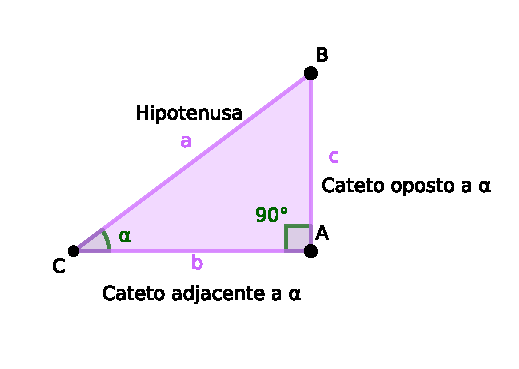
\includegraphics[width=7cm]{triangulo_retangulo.pdf}}
   \caption{Triângulo retângulo}
  \end{figure}
 para este triângulo temos que é válido o seguinte teorema:

 \vskip0.3cm

\colorbox{azul}{
 \begin{minipage}{0.9\linewidth}
 \begin{center}
 \textbf{Teorema de Pitágoras}
  \[a^2= b^2 + c^2.\]
 \end{center}
 \end{minipage}}

 \vskip0.3cm

 Este é um resultado importante, já que com ele é possível encontrar o valor de um dos lados do triângulo, nos casos em que não temos todos os lados dados, normalmente é utilizado para encontrar o valor da altura de um triângulo.

 Para este triângulo, as funções seno, cosseno e tangente são dadas pelas seguintes razões trigonométricas, nesta ordem:

 \vskip0.3cm

\colorbox{azul}{
 \begin{minipage}{0.9\linewidth}
 \begin{center}
 \textbf{Funções trigonométricas}
  \begin{eqnarray*}
   \sen(\alpha)= \frac{c}{a}= \frac{CO}{HI} \; \ \
   \cos(\alpha)= \frac{b}{a}= \frac{CA}{HI} \; \ \
   \tan(\alpha)= \frac{c}{b}= \frac{CO}{CA}.
 \end{eqnarray*}
 \end{center}
 \end{minipage}}

 \vskip0.3cm

 Como a soma dos ângulos internos de um triângulo é $180 \degree$, e estamos aqui tratando de um triângulo retângulo, decorre que neste caso $0 \degree \leqslant \alpha \leqslant 90 \degree$. Porém estas funções estão definidas para qualquer número real, mas para nosso estudo é suficiente conhecer seus valores para os ângulos $0 \degree \leqslant \alpha \leqslant 360 \degree$.

 Destacamos aqui os valores do seno, cosseno e tangente dos \emph{ângulos notáveis} que são os mais utilizados:

 \begin{table}[H]
 \centering
 \begin{tabular}{|c|c|c|c|c|c|} \hline
 \rowcolor{cinza}
               & $0 \degree$  & $30 \degree$  & $45 \degree$  & $60 \degree$ & $90 \degree$  \\\hline
  $\pmb{\sen}$ & $0$ &$\frac{1}{2}$ & $\frac{\sqrt{2}}{2}$ & $\frac{\sqrt{3}}{2}$ & $1$ \\\hline
  $\pmb{\cos}$ & $1$ & $\frac{\sqrt{3}}{2}$ & $\frac{\sqrt{2}}{2}$ & $\frac{1}{2}$ & $0$ \\\hline
  $\pmb{\tan}$ & $0$ & $\frac{\sqrt{3}}{3}$ & $1$ & $\sqrt{3}$ & $\nexists$ \\\hline
 \end{tabular}
\end{table}
 Na próxima seção veremos como utilizar estes valores para calcular seno, cosseno e tangente de ângulos maiores que $90 \degree$.

\section{Círculo Trigonométrico}

 No plano cartesiano, consideremos um círculo de centro na origem e raio $1$, neste círculo representamos as imagens das funções trigonométricas aplicadas à  $0 \degree \leqslant \alpha \leqslant 360 \degree$. Como mostra a seguinte figura:
 \begin{figure}[H]
   \centering
   \fbox{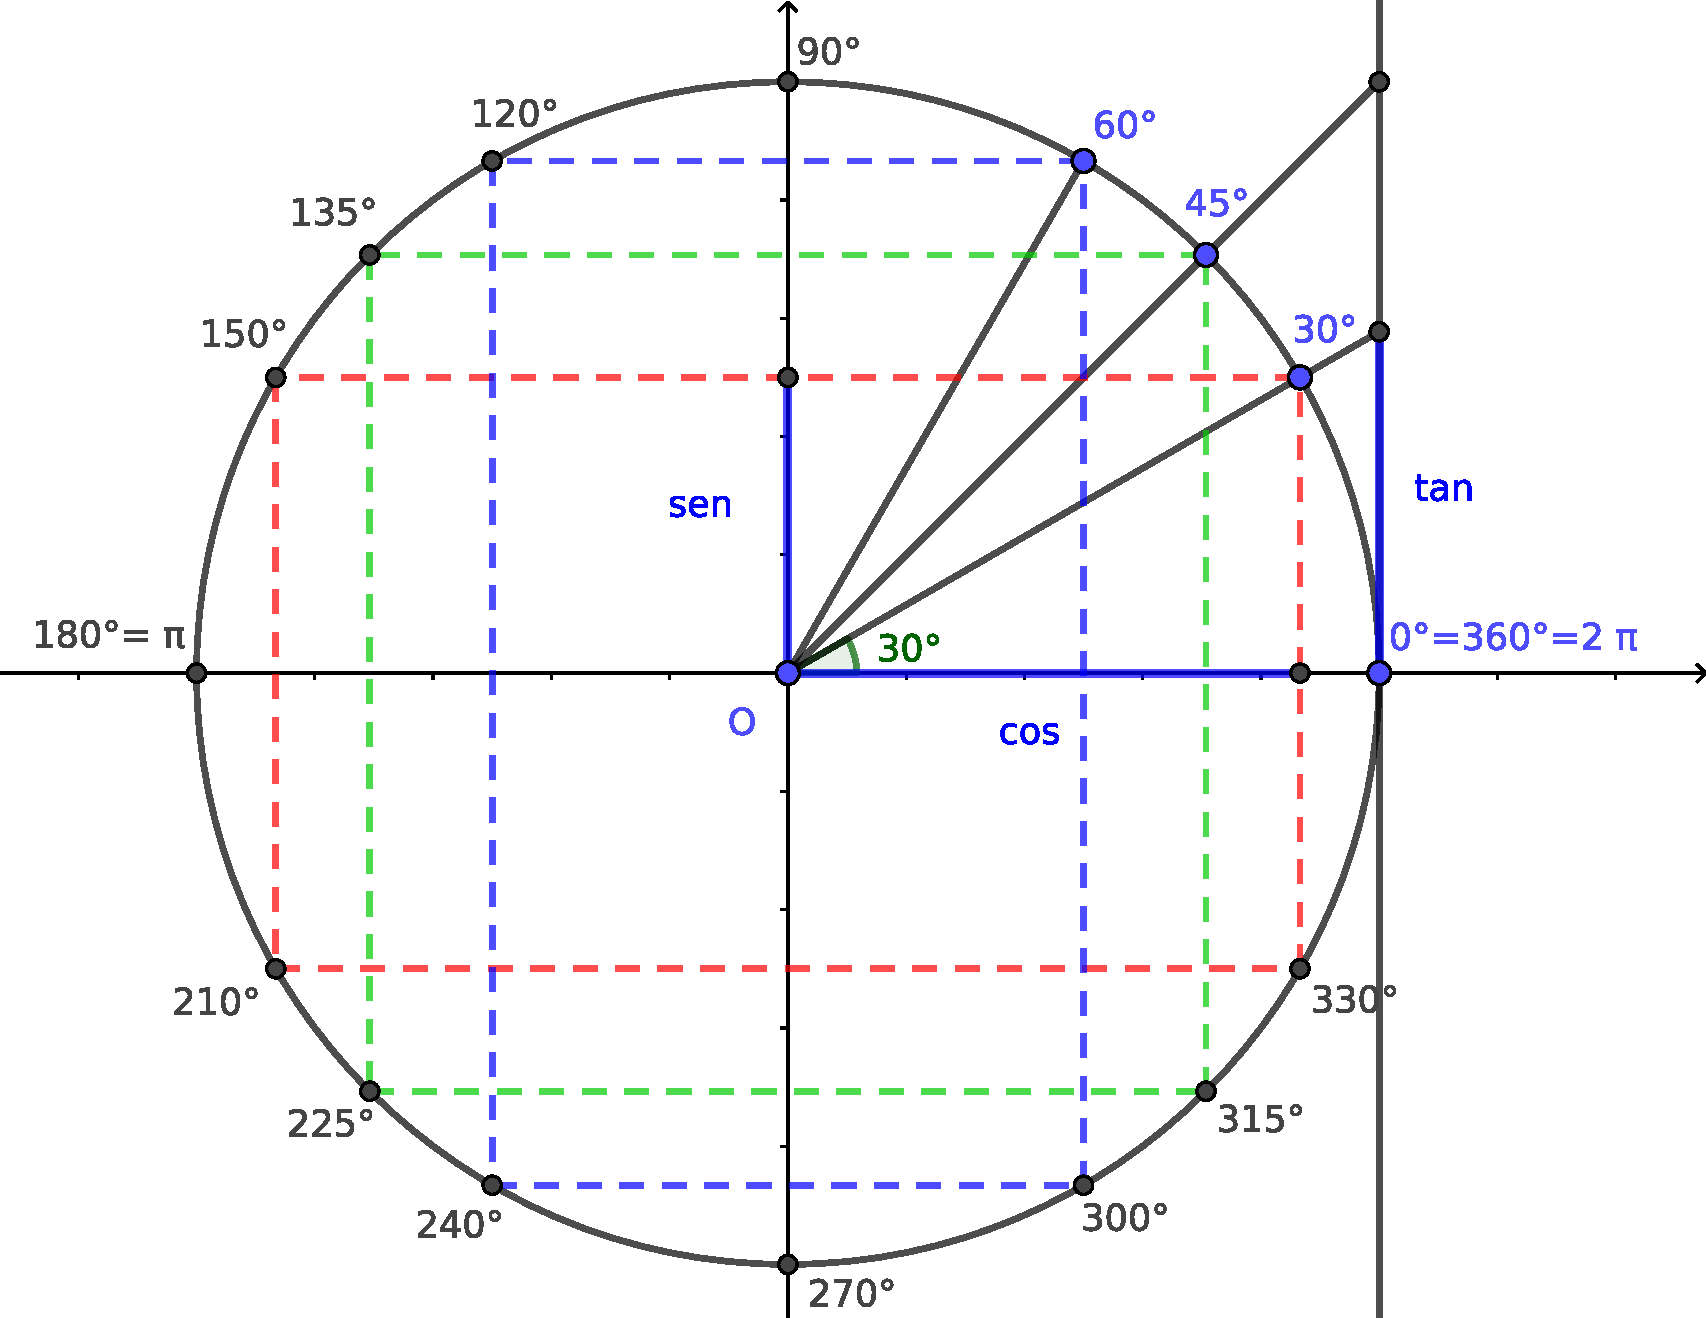
\includegraphics[width=9cm]{circulo_trigonometrico.pdf}}
   \caption{Círculo trigonométrico}
  \end{figure}

  A partir do círculo trigonométrico concluímos que:

  \begin{table}[H]
 \centering
 \begin{tabular}{|c|c|c|c|} \hline
 \rowcolor{cinza}
               &  $120\degree$  & $135\degree$  &  $150\degree$ \\\hline
  $\pmb{\sen}$ & $\sen(60\degree)$ &$\sen(45\degree)$ & $\sen(30\degree)$  \\\hline
  $\pmb{\cos}$ & $-\cos(60\degree)$ &$-\cos(45\degree)$ & $-\cos(30\degree)$  \\\hline
  $\pmb{\tan}$ & $-\tan(60\degree)$ &$-\tan(45\degree)$ & $-\tan(30\degree)$  \\\hline
 \end{tabular}
\end{table}

 \begin{table}[H]
 \centering
 \begin{tabular}{|c|c|c|c|} \hline
 \rowcolor{cinza}
                & $210\degree$ & $225\degree$  & $240\degree$  \\\hline
  $\pmb{\sen}$ &  $-\sen(30\degree)$ & $-\sen(45\degree)$ & $-\sen(60\degree)$  \\\hline
  $\pmb{\cos}$ &  $-\cos(30\degree)$ & $-\cos(45\degree)$ & $-\cos(60\degree)$  \\\hline
  $\pmb{\tan}$ &  $\tan(30\degree)$ & $\tan(45\degree)$ & $\tan(60\degree)$   \\\hline
 \end{tabular}
\end{table}

 \begin{table}[h]
 \centering
 \begin{tabular}{|c|c|c|c|} \hline
 \rowcolor{cinza}
               & $300\degree$ & $315\degree$ & $330\degree$ \\\hline
  $\pmb{\sen}$ & $\sen(60\degree)$ & $\sen(45\degree)$ & $\sen(30\degree)$ \\\hline
  $\pmb{\cos}$ & $\cos(60\degree)$ & $\cos(45\degree)$ & $\cos(30\degree)$  \\\hline
  $\pmb{\tan}$ & $-\tan(60\degree)$ & $-\tan(45\degree)$ & $-\tan(30\degree)$  \\\hline
 \end{tabular}
\end{table}


  Os ângulos podem também ser representados em radianos, respeitando a seguinte relação:

  \[\destaque{\pi \text{ radianos}= 180 \degree}\]

  Usando esta relação podemos transformar graus para radianos e radianos para graus, vamos ver dois exemplos:

  \begin{exem}
   Qual a medida em graus do ângulo que mede $\frac{\pi}{4} rad$?

   \underline{Resolução:}

   Sabemos que $\pi rad= 180\degree$, portanto usando a regra de 3 abaixo conseguimos encontrar o valor em graus deste ângulo:
   \begin{eqnarray*}
  \text{Graus} & & \text{Radianos} \\
   180 & = & \pi\\
  x & = & \frac{\pi}{4}
 \end{eqnarray*}
 usando a propriedade da proporcionalidade, ou seja, multiplicando cruzado temos:

 $180 \cdot \frac{\pi}{4}= \pi \cdot x \Rightarrow \pi \cdot x= \frac{180 \pi}{4} \Rightarrow x= \frac{45 \pi}{\pi} \Rightarrow x= 45\degree$.

 \fim
  \end{exem}

  \begin{exem}
   Qual a medida em radianos do ângulo que mede $30\degree$?

   \underline{Resolução:}

   Sabemos que $\pi rad= 180\degree$, portanto usando a regra de 3 abaixo conseguimos encontrar o valor em graus deste ângulo:
   \begin{eqnarray*}
  \text{Graus} & & \text{Radianos} \\
   180 & = & \pi\\
  30 & = & x
 \end{eqnarray*}
 usando a propriedade da proporcionalidade, ou seja, multiplicando cruzado temos:

 $180 \cdot x= \pi \cdot 30 \Rightarrow x= \frac{30 \pi}{180} \Rightarrow x= \frac{\pi}{6} rad$.

 \fim
  \end{exem}



 \section{Relações trigonométricas}

 Só a critério de conhecimento, segue uma lista de algumas relações trigonométricas que são interessantes pela grande quantidade de aplicações:

 \begin{eqnarray*}
  \tan(x)&=&\frac{\sen(x)}{\cos(x)} \\
  \sen^2(x) + \cos^2(x)&=&1 \\
  \sen(a+b)&=&\sen(a)\cdot \cos(b)+\sen(b)\cdot \cos(a) \\
  \sen(a-b)&=&\sen(a)\cdot \cos(b)-\sen(b)\cdot \cos(a) \\
  \cos(a+b)&=&\cos(a)\cdot \cos(b)-\sen(a)\cdot \sen(b) \\
  \cos(a-b)&=&\cos(a)\cdot \cos(b)+\sen(a)\cdot \sen(b) \\
  \tan(a+b)&=& \frac{\tan(a)+\tan(b)}{1-\tan(a)\cdot \tan(b)} \\
  \tan(a-b)&=& \frac{\tan(a)-\tan(b)}{1-\tan(a)\cdot \tan(b)}
 \end{eqnarray*}

\end{document}